\chapter{Анализ литературы, патентов и обзор практики рецикла урана}\label{ch:ch1}

\section{Теоретические основы}

% \subsection{Основы теории разделения в каскадах}
% \textcolor{red}{Базовые понятия (разделительный элемент, симметричн.-противоточное соединений, каскад) + основные уравнения (балансы, срез, коэффициенты разделения ступеней)}

% \dots

% \subsection{Модельные каскады}

% Тогда как обогащение природного урана можно свести к простой задаче разделения бинарной смеси, обогащение переработанного урана является задачей разделения изотопов многокомпонентной изотопной смеси.
% % А сложность расчетов молекулярно-селективного переноса для многокомпонентных изотопных составов заключается в необходимости использования математических моделей для разделения многокомпонентных изотопных смесей (хотя это касается и разделения неурановых химических элементов, например вольфрама).

% \subsubsection{Модель симметрично-противоточного каскада}

% Модели, которые будут рассмотрены в данном разделе -- «квазиидеальный» каскад, R-каскад, поступенный расчет -- вытекают из модели симметрично-противоточной коммутации ступеней каскада.

% \dots

% Вычислительные эксперименты, проводимые с целью исследования каскадов, опираются на использование специальных математических моделей, которые будут представлены в текущем разделе. Они позволяют заметно упростить изучение закономерностей изотопно-селективного массопереноса в разделительных каскадах. Этот вспомогательный инструмент принято называть модельным каскадом.

% Физико-математические модели каскадов основанны на фундаментальных законах, таких как закон сохранения вещества.
% Эти теоретические описания адекватны процессу разделения в реальных каскадах, состоящих из тысяч разделительных аппаратов.
% В качестве разделительных аппаратов сегодня, как правило, используются газовые центрифуги.

% В области математического моделирования разделительных каскадов на сегодня разработан обширный набор расчетных моделей, которые могут быть применены в том числе и к задаче обогащения регенерированного урана.
% В нашем случае для моделирования физического процесса разделения изотопов урановой смеси может быть применен ряд специальных математических моделей.

% Наиболее общая из таких моделей называется «квазиидеальным» каскадом, где предполагается постоянство относительных коэффициентов разделения, а также срезов парциальных компонентов по каскадным ступеням \cite{yamamotoMulticomponentIsotopeSeparating1978}.
% В настоящее время он используется в двух приближениях: со слабым обогащением (Q-каскад \cite{borisevichNewApproachOptimize2011, kolokoltsovDesignCascadesSeparating1970, zengQCascadeExplanation2012}) и произвольным обогащением (квазиидеальный каскад \cite{sulaberidzeSpecialFeaturesEnrichment2006}).
% Применение модельных каскадов значительно упрощает как анализ закономерностей массообмена в каскаде для многокомпонентного разделения, так и соответствующий расчет.
% В исследованиях, как правило, когда обогащенный переработанный уран обогащается многопоточными схемами, часто используется модель R-каскада (Matched Abundance Ratio Cascade-MARC \cite{kazukihidaSimultaneousEvaluationEffects1986, delagarzaMulticomponentIsotopeSeparation1961, woodEffectsSeparationProcesses2008}).
% Это особый случай `квазиидеального' каскада. Здесь условие отсутствия смешивания выполняется для выбранной пары компонентов (например, это могут быть изотопы $^{235}$U и $^{238}$U).
% Еще раз подчеркнем, что все вышеупомянутые каскадные модели действуют как физически эквивалентные представления и, как показано в \cite{sulaberidzeClassificationModelCascades2020}, могут быть выведены из <<обобщенного модельного каскада>>, которым является симметрично-противоточный каскад с постоянными по его длине относительными коэффициентами разделения).

% \subsubsection{Модель «квазиидеального» каскада}
% \dots

% \subsubsection{Каскад с несмешиванием относительных концентраций двух заданных компонентов смеси (R-каскад)}
% \dots

% \subsubsection{Поступенный расчет}
% \dots

% \subsection{История развития модельных каскадов}
% Работе по поиску схем для обогащения регенерата предшествовали разработки математического аппарата для моделирования разделения многокомпонентных смесей \cite{delagarzaMulticomponentIsotopeSeparation1961}.
% Изначально, эта идея рассматривалась для газодиффузионного метода разделения, которая в последующем была адаптирована для метода газовой центрифуги с характерным б'ольшим коэффициентом разделения \cite{yamamotoMulticomponentIsotopeSeparating1978}.
% Проходя через основные вехи развития модельных каскадов для моделирования многокомпонентных изотопных смесей, в работе \cite{delagarzaMulticomponentIsotopeSeparation1961} предложена модель R-каскада, а в \cite{levin1963} -- М*-каскада.
% Затем в \cite{kolokoltsovDesignCascadesSeparating1970} разработана модель Q-каскада, а в \cite{sazykinKvaziidealnyeKaskadyDlya2000} -- квазиидеального.

\subsection{Истоки возникновения проблемы с $^{232,234,236}$U}

В конечном товарном продукте -- низкообогащенном уране -- регламентировано содержание изотопов четного ряда -- $^{232,234,236}$U.
Наличие строгих ограничений обсуловлено нейтронно-физическими и радиационными свойствами четных изотопов $^{232,234,236}$U \cite{smirnovEvolutionIsotopicComposition2012, proselkovAnalizVozmozhnostiIspolzovaniya2003, dudnikovInfluence236UEfficacy2016}.
Эти изотопы, возникшие при облучении топлива и в ходе последующего его хранения, не могут быть извлечены в ходе переработки из урановой смеси. Они могут быть удалены только с использованием технологий разделения изотопов, что и затрудняет обогащение регенерированного урана для его возврата в ЯТЦ.

Так, первый в этом ряду изотоп $^{232}$U является родоначальником длинной цепочки распада, в которую входят нуклиды-излучатели жёстких гамма-квантов.
Основным дочерним источником интенсивного гамма-излучения (2.6 МэВ) является короткоживущий $^{208}$Tl ($t_{\frac{1}{2}}=3.65$ мин.) \cite{matveevUran232EgoVliyanie1985,abbasProliferationResistanceFeatures2013}. Опасность на производстве также представляет еще один дочерний изотоп -- $^{220}$Rn (торон) вследствие его эманирования в воздух рабочей зоны.

$^{232}$U вместе $^{234}$U превносят альфа-частицы в смесь гексафторида урана ($UF_6$ -- соединение, используемое в процессе обогащения урана \cite{orlovWayObtainUranium2015, orlovDesublimationPurificationTransporting2017}), вероятно, приводя к его диссоциации, что может привести к нежелательному появлению и дальнейшему осаждению в каскаде легких компоненты, таких как, например свободный фтор ($F_2$) \cite{kryuchkovObogashchennyyUranDobavleniem2007, bernhardtRadiationEffectsAlpha1958, shmelevRazrabotkaRaschetnoyModeli2012}.

$^{236}$U, являясь паразитным поглотителем нейтронов, препятствует развитию цепной реакции.
Этот эффект отравления реактора должен быть скомпенсирован дополнительным количеством делящегося $^{235}$U в топливе.
То есть, для обеспечения требуемого эквивалента уровня обогащения по $^{235}$U, к заданной концентрации $^{235}$U в продукте для случая обогащения природного урана необходимо обеспечить добавку делящегося $^{235}$U.
Ее величина определяется наличием $^{236}$U:
$C_{235 экв.}^{P}=C_{235 прир.}^{P}+\Delta C_{235}$, где $\Delta C_{235}$ соответствует некоторой функции $f\left(C_{236}^{P}\right)$, которая в простейшем случае является линейной вида $K_{236} \times C_{236}^{P}$. $K_{236}$ называют коэффициентом компенсации реактивности. Его значение значение в зависимости от (типа реактора и топливной кампании?) может лежать в пределах 0.2--0.6 \cite{delagarzaMulticomponentIsotopeSeparation1961, delculAnalysisReuseUranium2009}. 

$^{234}$U имеет тенденцию захватывать нейтрон и превращаться в делящийся $^{235}$U, что должно уменьшить необходимую компенсацию $^{236}$U \cite{dyachenkoIspolzovanieRegenerirovannogoUrana2012}, что в расчетах не учитывается ввиду порядка малости.

Содержание этих изотопов в низкообогащенном продукте может регулироваться различными стандартами, такими как, например, ASTM C996 - 15 \cite{c26committeeSpecificationUraniumHexafluoride}.

\subsection{Задача обогащения регенерированного урана с точки зрения разделительных технологий}

Специфика задачи обогащения регенерированного урана заключается в том, что она представляет собой более сложную разделительную проблему.
Это обусловлено тем, что, в отличие от случая обогащения природного урана, регенерированный уран представляет собой многокомпонентную смесь и, помимо обогащения целевого изотопа -- $^{235}$U, необходимо одновременно выполнять ограничения на еще три изотопа -- $^{232}$U, $^{234}$U и $^{235}$U.
Таким образом, при решении задачи обогащения регенерата необходимо обеспечить:
\begin{enumerate}
  \item Соответствие произведенного низкообогащенного урана необходимым требованиям (спецификациям), которое может быть сформулировано как удовлетворение ограничения на присутствие нежелательных "четных" изотопов урана. Так, в соответствии с распространенными стандартами для низкообогащенного урана:
  \begin{enumerate}
    \item концентрация изотопа $^{232}$U в низкообогащенном уране строго ограничена величиной $5\cdot10^{-7}$\%, или, в некоторый случаях, $2\cdot10^{-7}$\% и $1\cdot10^{-7}$\% \cite{smirnovKaskadnyeShemyZadachah2012, c26committeeSpecificationUraniumHexafluoride}.
    \item Отношение концентраций изотопов $^{234}$U и $^{235}$U в продукте не должно превышать 0.02.
    \item $^{236}$U должен быть скомпенсировано дополнительным количеством делящегося $^{235}$U в низкообогащенном уране.
  \end{enumerate}
  \item Использование восстановленного урана на единицу продукта НОУ в необходимой пропорции ($\approx$0.93), что соответствует возврату в топливный цикл в виде 1 кг свежего топлива 1 кг ОЯТ. Такое условие может быть связано с мерами контроля оборота делящихся материалов, что особенно актуально для экспорта ядерного топлива. Величина  $\approx$0.93 соответствует доле извлекаемой в ходе переработки ОЯТ урановой фракции.
  \item Вовлечение в топливный цикл максимально возможной доли изотопа $^{235}$U для повышения экономии природного урана
\end{enumerate}

Также могут иметь место следующие условия:
\begin{enumerate}
  \item Вывод из топливного цикла изотопов $^{232,234,236}$U, который можно обеспечить только посредством изотопного разделения. Концентрации этих нежелательных искусственных изотопов должны быть минимизированы в условиях многократной переработки урановой составляющей топлива. Это важно чтобы избежать их накопления к последующим рециклам.
  \item Предотвращение нежелательных потерь работы разделения в ходе операции разделения изотопов. Такие потери могут быть связаны с недостатками каскадных схем, когда осуществляется смешение изотопных составов с различными концентрациями $^{235}$U. 
  \item Избежание накопления нештатных (высокотоксичных) отходов -- побочных продуктов с высокой концентрацией изотопов $^{232,234}$U. К тому же, в них теряется $^{235}$U.
  \item Предел допустимой концентрации $^{235}$U на любом из стадий производства может быть ограничен лицензией обогатительного комбината.
  \item Предел доступных для решения задачи разделительных мощностей.
  \item Ограничения на расход сырья разбавителя, которым может быть как природный уран, так и обедненный или предварительно подготовленный НОУ.
\end{enumerate}

Политика вовлечения регенерированного урана в ЯТЦ позволяет достигать экономии природного урана на уровне 11--20\% и многократного снижения объемов высокоактивных радиоактивных отходов за счет переработки ОЯТ \cite{delculAnalysisReuseUranium2009}. Возможность же осуществлять многократный рецикл урана и курс на удлинение (пролонгацию) топливных кампаний, связанный с повышением исходного уровня обогащения, открывает перспективы еще б`ольших преимуществ повторного использования делящегося материала.
Все это делает актуальным разработки каскадных обогатительных схем, позволяющих эффективно использовать регенерированный уран при производстве товарного НОУ с учетом всех описанных выше требований и ограничений как в условиях однократного, так и многократного рецикла урана.


\section{Промышленный опыт}\label{sec:ch1/sec1}
Промышленный опыт замыкания ЯТЦ опирается на технологии переработки ОЯТ и последующего рецикла ядерных материалов.
В России имеется уникальный технологический задел, связанный с переработкой ОЯТ \cite{balihinSostoyaniiPerspektivahRazvitiya2018}.
Таким образом, заключительная часть ЯТЦ (back-end) является перспективным направлением развития международного бизнеса Росатома \cite{efimenkoProblemyPerspektivyRazvitiya2017}. 

Что касается рецикла ядерного топлива, зарубежный опыт исторически базируется на однократном использовании MOX-топлива.
В данной работе будем опираться на Российский опыт возврата топлива в ЯТЦ \cite{international2003iaea}.
К тому же, по части повторного использования урановой составляющей, отечественную ядерную индустрию можно считать глобальным лидером.
Эта практика вовлечения регенерата урана в топливные циклы энергетических реакторов базируется на смешении регенератов урана, извлекаемых из ОЯТ ВВЭР и ОЯТ транспортных реакторов с высоким содержанием $^{235}$U.
Такая схема реализована для производства исходного сырья для изготовления топлива РБМК на заводе РТ-1 \cite{volkVozvratUranaIz2010}.
Более того, этот вариант также апробирован для изготовления опытных тепловыделяющих сборок (ТВС) для реакторов ВВЭР \cite{proselkovAnalizVozmozhnostiIspolzovaniya2003}, требующих более высокого уровня обогащения.

На сегодняшний день для широкомасштабного использования регенерированного урана существует ряд препятствий, состоящих в ограничениях мощностей переработки ОЯТ, ограниченном опыте промышленной эксплуатации топлива на основе обогащенного регенерата, неготовности фарбрикационного, радиохимического и сублиматного производств вводить производственные линии для материала с повышенной радиотоксичностью (отсутствие у последних двух лицений на работу с материалом >1\% $^{235}$U), а также неисследованный вопрос хранения ОГФУ с $^{232,234}$U.

При этом, опираясь на передовой уровень разделительной технологии, можно заключить, что задача обогащения регенерата до необходимого для повторного использования в энергетических ядерных реакторах уровня концентрации изотопа $^{235}$U может быть решена.
Сложившаяся к текущему моменту научно-производственная база и лидирующие объемы имеющихся в нашей стране промышленных разделительных мощностей, основанных на центробежном методе разделения, являются основным аргументом в пользу готовности к вовлечению регенерата в топливный цикл легководных реакторов.
Однако, ввиду долгосрочных планов отрасли по замыканию ЯТЦ и развитию международных топливных поставок, необходимо предполагать необходимость  многократного рецикла и наличие дополнительных ограничений на расход материалов.


\section{Задача поиска оптимальной схемы}

Перейдем к вопросу подбора каскадной схемы для производства НОУ, способной обеспечить наилучшее решение с точки зрения выбранных критериев.
Такими критериями обычно выступают показатели, называемые интегральными в теории разделения изотопов: расход природного урана и затраты работы разделения.
Они подлежат минимизации, однако зачастую являются конкурирующими.
В качестве целевой функции можно рассматривать аддитивный критерий стоимости или энергозатрат, который может включать в себя, помимо расхода природного урана и затрат работы разделения, расходы (стоимостные или энергетические) на утилизацию нештатных отходов, а также на прочие вовлекаемые (в качестве потоков питания) материалы, например ОГФУ, для которого такой показатель может быть отрицательным.

Следует напомнить, что задача при этом должна быть решена в рамках набора заданных условий, а это накладывает ограничения на оптимизацию целевых показателей.
К тому же, могут возникнуть дополнительные факторы, которые могут претендовать на роль первостепенных показателей эффективности.
Ими могут быть минимум нештатного отхода, минимизация загрязнения резделительного оборудования.

\section{Расчетная модель}

В данной работе будут использованы математические модели  `квазиидеального' каскада и его частный случай -- R-каскад. Расчеты будут проведены в предположениях симметрично-противоточной схемы коммутации, а также при одинаковом коэффициенте разделения $q$ на каждой ступени. При этих условиях R-каскад можно считать эквивалентным `квазиидеальному' \cite{zengRelationshipNonmixingCascade2020}.

\section{Сравнительный анализ известных схем}

История теоретических исследований вопроса повторного использования урана в ядерном топливе насчитывает около полувека.
В этом разделе будет рассмотрена эволюция методик, предложенных для решения задачи обогащения регенерированного урана с целью его возврата в топливный цикл энергетических реакторов.
Развитие подходов к вовлечению регенерата в производство низкообогащенного урана можно проследить через историю совершенствования предлагаемых каскадных схем.
Для каждой рассмотренной схемы будет проведен критический анализ, выявляющий ее достоинства и недостатки.

\subsection{Основные модификации ординарного каскада}

Непосредственное применение простейшей схемы -- ординарного каскада, используемого для обогащения природного урана имеет существенные ограничения в рамках поставленной нами задачи.
В условиях многократного рецикла, она не позволяет добиться желаемого результата, ввиду наличия ограничений на присутствие в конечном продукте -- низкообогащенном уране -- четных изотопов.
Такое ограничение и подтолкнуло исследователей к развитию подходов к производству НОУ из обогащенного регенерата с учетом заданных требований.
В работах \cite{sulaberidzeNekotoryhRazdelitelnyhProblemah2004,sulaberidzeProblemsRefinementRecycled4, smirnovKaskadnyeShemyZadachah2012} было показано, что отрицательное влияние указанных изотопов делает непригодным для обогащения регенерата ординарный каскад (каскад, имеющий три внешних потока – питание, отбор и отвал), используемый для обогащения природного урана. Это происходит, поскольку при обогащении регенерата по $^{235}$U в таком каскаде, в отборе, помимо $^{235}$U неминуемо будут концентрироваться все легкие компоненты, в первую очередь $^{232}$U. Поэтому ординарный каскад применим только для обогащения относительно «чистого» состава регенерата, в котором содержание $^{232}$U меньше допустимой нормы на порядок и более, что нехарактерно для большинства изотопных составов выгружаемого из активной зоны ВВЭР облученного топлива \cite{bormanTehnikoekonomicheskiyAnalizVozmozhnyh2012}.

Рассмотрим же технические решения, позволяющие корректно (соблюдая вышеозначенные условия) решить задачу обогащение регенерата. Начнем с ряда схем, основанных на ординарном (трехпоточном) каскаде.
Его можно применять, например, следующими способами (рис. \ref{fig:diagram1}) \cite{smirnovKaskadnyeShemyZadachah2012}:
\begin{enumerate}
  \item Добавление смеси регенерированного урана к природному урану перед подачей в каскад рис. (рис. \ref{fig:diagram1}.1).
  \item Получение обогащенной фракции из регенерата и последующее ее разбавление природной урановой смесью (рис. \ref{fig:diagram1}.2 ).
  \item Подготовка смеси НОУ из природного урана немного больше, чем необходимо для получения товарного НОУ требуемого качества, с последующим разбавлением его регенератом (рис. \ref{fig:diagram1}.3 ).
\end{enumerate}

\begin{figure}[ht]
  \centerfloat{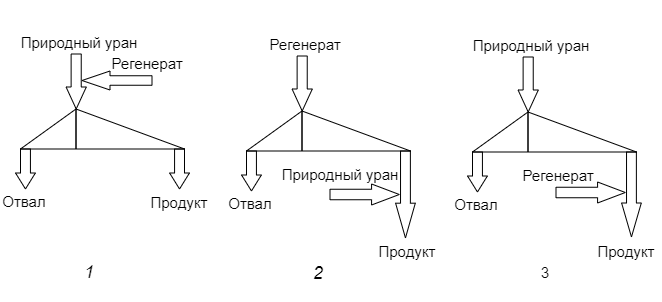
\includegraphics[scale=0.7]{cascades/diagram1}}
  \caption{Схемы на основе ординарного каскада}\label{fig:diagram1}
\end{figure}

Для всех вариантов схем рис. \ref{fig:diagram1} сотношение между расходом регенерата и разбавителем природного происхождения определяется пределом допустимой концентрации $^{232}$U в конечном продукте -- низкообогащенном уране. Также делается поправка на необходимость компенсации отрицательной реактивности $^{236}$U. В то же время концентрация $^{235}$U не должна быть ниже, чем требуется для НОУ с определенными свойствами.

Основным преимуществом таких схем является простота реализации, поскольку нет необходимости в модификации устройства каскада -- операции разбавления осуществляются за пределами  ординарного каскада.
При этом, как недостаток можно выделить потери работы разделения, возникающие из-за смешения потоков с различными изотопными концентрациями $^{235}$U.
Также эти схемы не могут обеспечить полный возврат ОЯТ в ЯТЦ.
Однако такие схемы не пригодны для решения задачи вовлечения регенерата в условияx многократного рецикла, что будет в очередной раз продемонстрировано в данной диссертационной работе.

Рассмотрим вариант схемы, рис.\ref{fig:diagram1}.2, лучшим образом подходящий для задачи возврата регенерата урана второго рецикла (NET).

Схема рисунка \ref{fig:diagram1}.2 представляет собой возможный способ снижения накопления четных изотопов в регенерате урана \cite{SposobIzotopnogoVosstanovleniyaa}. Разбавление осуществляют следующим образом: сначала из регенерата в ординарном каскаде получают высокообогащенный уран (ВОУ), который затем разбавляют смесью, не содержащей минорных изотопов, добиваясь нужного содержания изотопа $^{235}$U в финальном продукте-низкообогащенном уране. Например, таким разбавителем может быть природный уран или отвалы разделительного производства. Для обогащения по изотопу $^{235}$U перед последующим разбавлением предложена массовая концентрация $\approx$36\% \cite{SposobIzotopnogoVosstanovleniyaa}. Практическое использование данной схемы ограничивают следующие недостатки: 
\begin{enumerate}
  \item потери работы разделения при разбавлении ВОУ (количественные оценки величин затрат работы разделения для рассматриваемой схемы будут представлены в разделе ... .
  \item ухудшение радиационной обстановки из-за загрязненности разделительного оборудования примесными изотопами, в частности $^{232}$U, ухудшающим радиационную обстановку.
  \item необходимость обогащения материала до уровня высокообогащенного урана, когда концентрация изотопа $^{235}$U превышает 20\%.
  Такой подход может иметь ограничения со стороны регулятора -- обогатительный комбинат может быть не в праве нарабатывать материал с такой высокой концентрацией $^{235}$U -- ввиду режима нераспространения.
\end{enumerate}

Как будет показано в разделе ..., базовые модификации ординарного каскада не способны решить задачу возврата в ЯТЦ регенерированного урана в условиях многократного рецикла.
Причем это невозможно даже если пренебречь нормативным ограничением на производство ВОУ.
Таким образом, рассмотрение приведенного ряда модификаций ординарного каскада подталкивает к дальнейшим поискам схем, которые бы нивелировали перечисленные недостатки.
Ниже дан критический анализ модификаций каскадных схем для обогащения регенерированного урана, основанных на использовании одиночных каскадов, имеющих дополнительные внешние потоки и двойных каскадов.

\subsection{Каскады с дополнительными внешними потоками (многопоточные схемы)}

Под внешними потоками следует понимать потоки, подаваемые в качестве питания каскада, а под внутренними -- потоки, циркулирующие внутри каскада. 

\subsubsection{Применение дополнительного потока-разбавителя}

Предожена схема с дополнительным потоком питания в виде регенерата, который подают на отдельную ступень рис. \ref{fig:2_inputs}) \cite{sulaberidzeQuasiidealCascadesAdditional2006}.
\begin{figure}[ht]
  \centerfloat{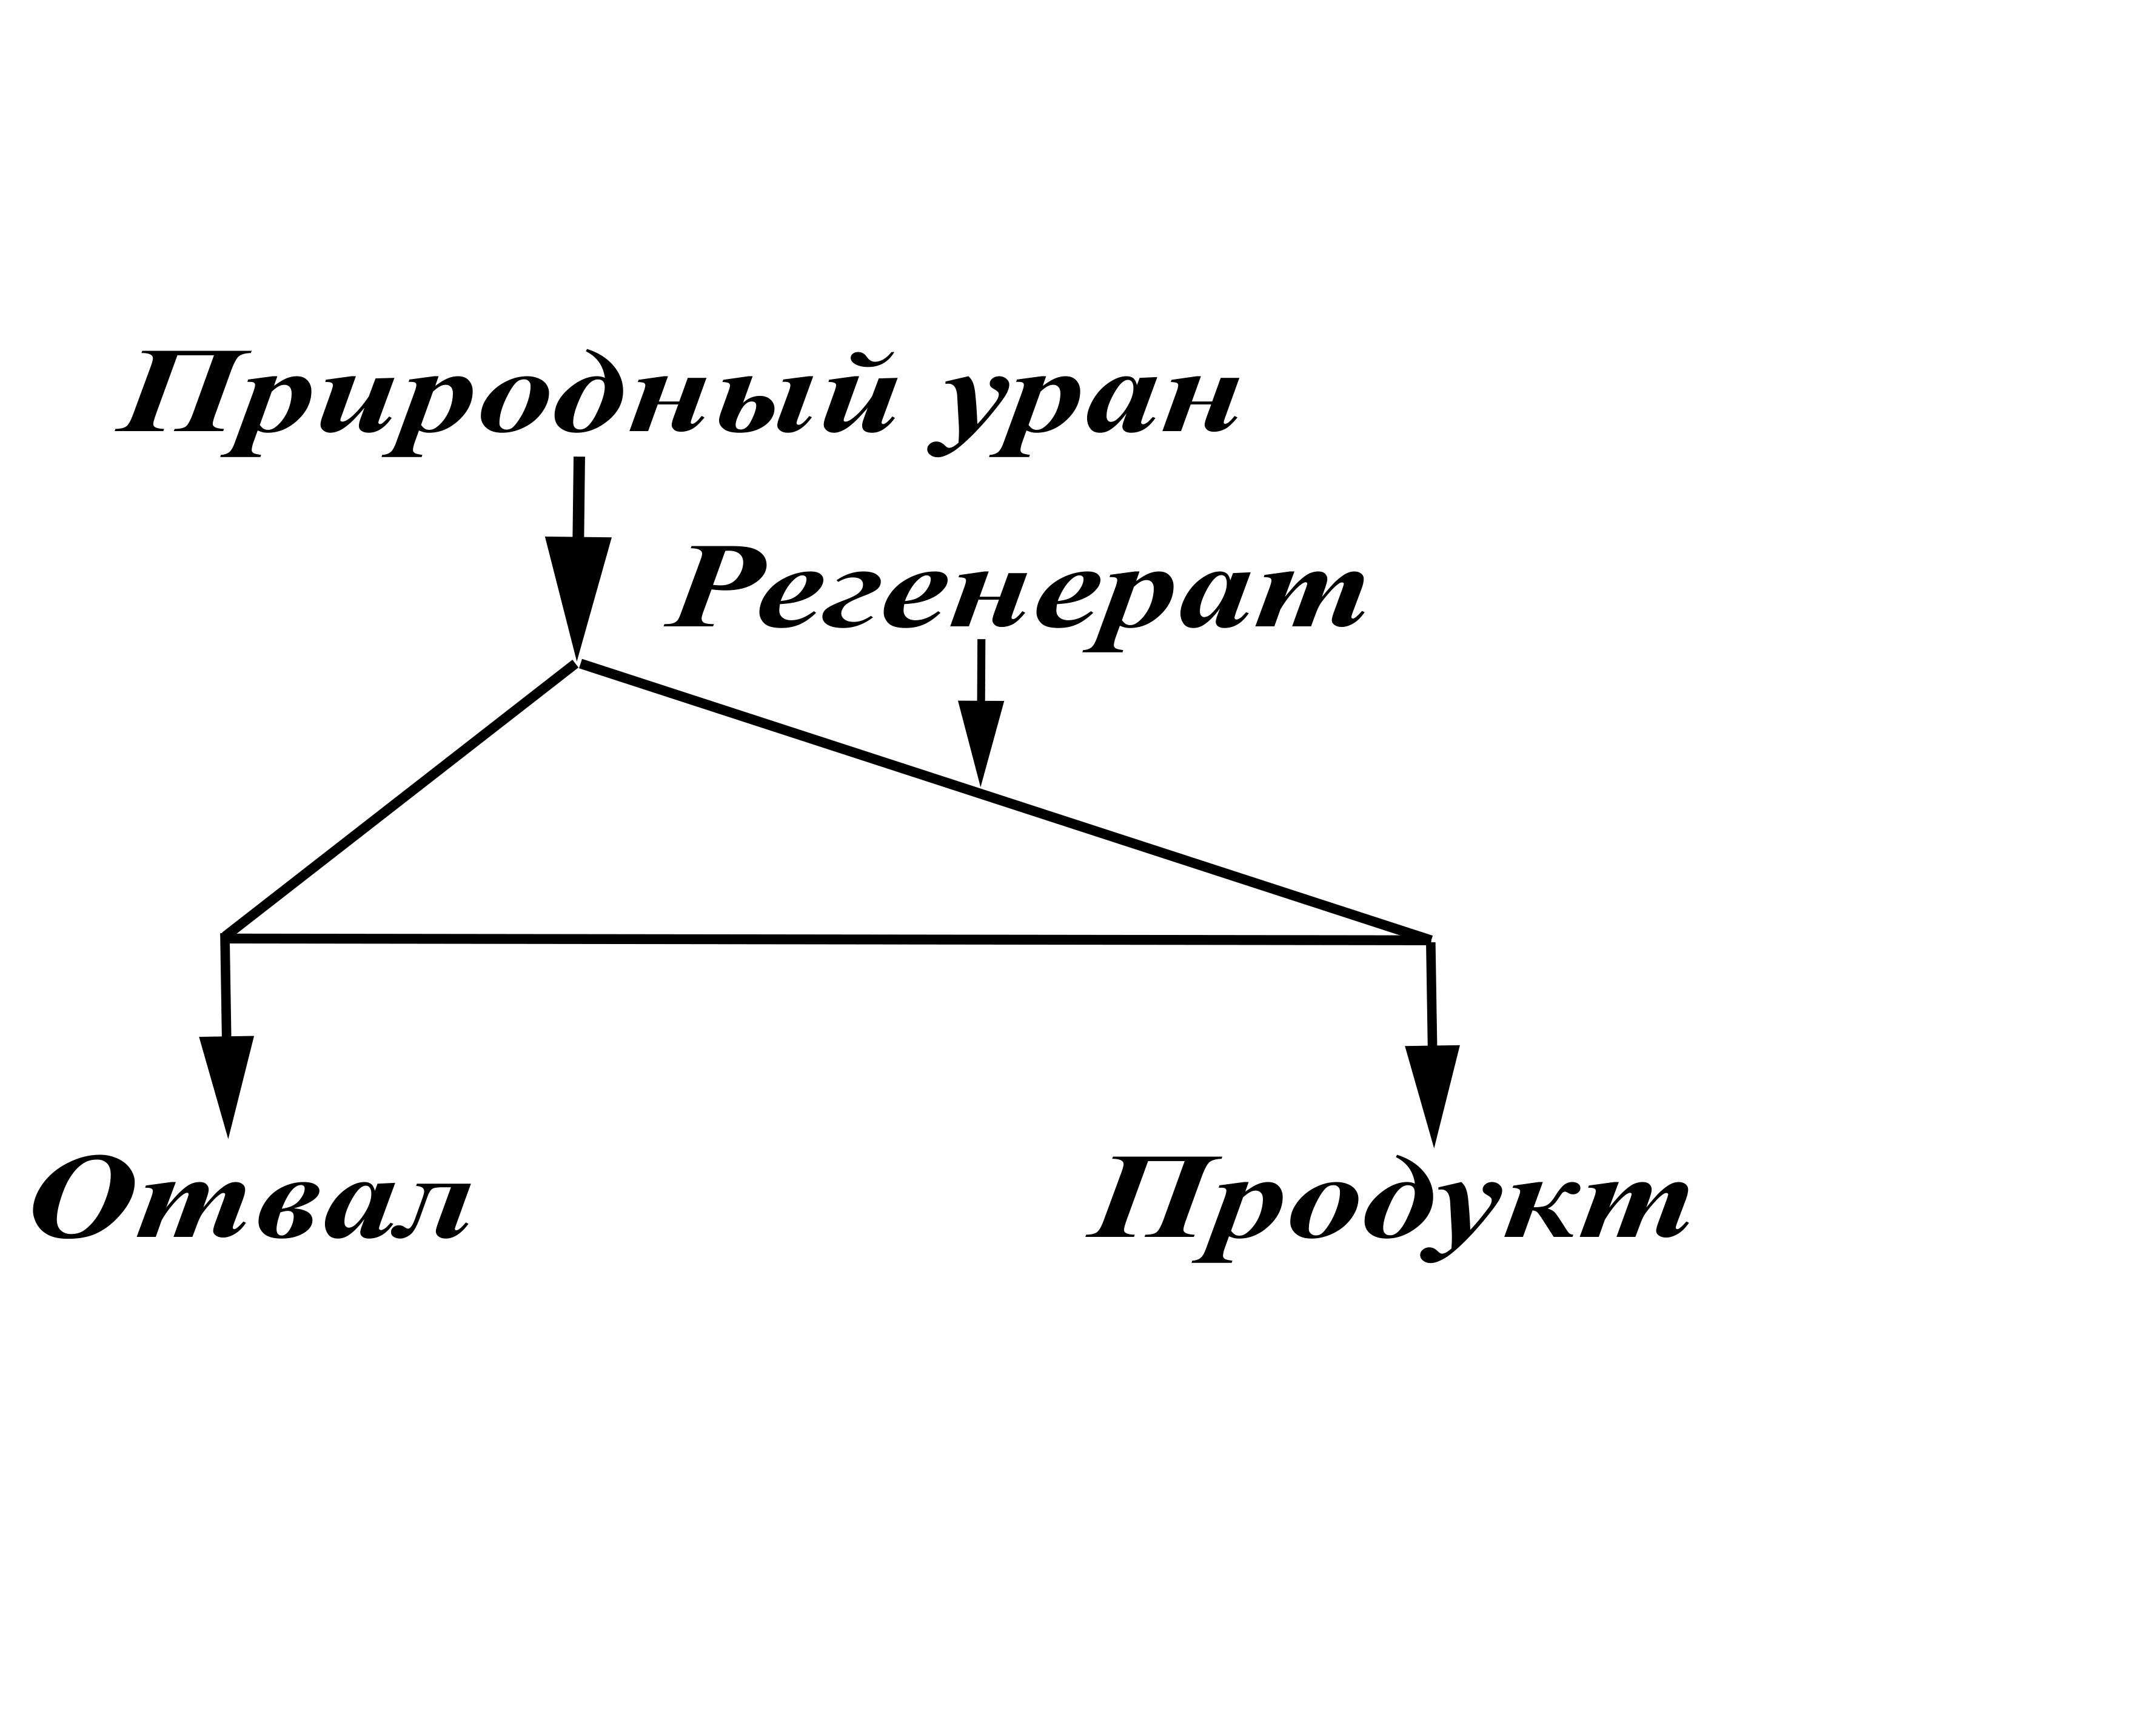
\includegraphics[scale=0.07]{cascades/2in}}
  \caption{Каскад с дополнительным потоком питания}\label{fig:2_inputs}
\end{figure}

Этот метод позволяет избежать потери работы разделения в ходе смешения потоков с различными концентрациями $^{235}$U, располагая дополнительный входной поток там, где концентрации внешнего и внутреннего потоков в $^{235}$U совпадают.
Отсюда, преимущество схемы с дополнительным потоком питания по сравнению с предыдущими обычными схемами, связано с отсутствием потерь работы разделения \cite{smirnovKaskadnyeShemyZadachah2012, sulaberidzeQuasiidealCascadesAdditional2006}.

Однако общим недостатком всех вышеупомянутых схем (рис. \ref{fig:diagram1} и \ref{fig:2_inputs}), является необходимость использования большого количества природного урана.
Вне зависимости от их устройства, для решения поставленной задачи, необходимо осуществлять разбавление регенерата существенным количеством природного урана, в несколько раз превышающим долю используемого регенерата. Это необходимо, прежде всего, чтобы снизить содержание $^{232}$U в продукте.
Тем не менее, при повторном использования топлива ВВЭР, даже такой подход может обеспечить значительную экономию природного урана $\approx$16\% уже на первом рецикле.
Суммарная же экономия природного урана за всю серию рециклов будет складываться из уменьшающихся с каждым рециклом показателей сэкономленного природного сырья. 
Применение же многократного рецикла, позволяет и дальше, используя материалы повторно, частично замещать расход природного ресурса \cite{colemanEvaluationMultipleSelfrecycling2010}), как показано в оценках в \cite{smirnovEvolutionIsotopicComposition2012}.

Проблема необходимости обеспечивать питание каскада преобладающим количеством природного урана , чтобы, в сущности, "разбавлять" четные изотопы  $^{232,234}$U, содержащиеся в регенерате, идет бок о бок с невозможностью обеспечить условие "полного" возврата выгоревшего топлива в ЯТЦ.
Для рассмотренных схем, такое условие, заключающееся в использовании 1 кг ОЯТ на 1 кг НОУ продукта, достижимо только для изотопных составов первого (иногда второго) рецикла топлива легководного реактора.
Таким образом, с помощью такой схемы нельзя обеспечить заданую пропорцию вовлечения регенерированного урана в условиях многократного рецикла \cite{smirnovApplyingEnrichmentCapacities2018}.
На примере рассматриваемого каскада с двумя питаниями, начиная с третьего цикла, расходовать требуемый уровень регенерата становится невозможно из-за ухудшения изотопного состава урана и наличия ограничений на изотопы $^{232,236}$U.

Так, в \cite{smirnovApplyingEnrichmentCapacities2018} были рассчитаны основные показатели, характеризующие экономику разделительного процесса: расход природного урана и затраты работы разделения (РР).
Было показано, что для каждого из первых двух циклах можно достичь экономии природного урана на уровне $\approx$20\%. Затем, этот показатель ухудшается, так как при заданных условиях, к третьему циклу повторного использования происходит значительная деградация изотопного состава.
Чтобы повысить пределы экономии природного урана, необходимо искать альтернативный разбавитель. Например, таким материалом может послужить обедненный уран (так называемые «хвосты» (или отвалы) -- побочный продукт процесса обогащения).
Он может быть эффективно использован для частичной замены природного урана в качестве основного разбавителя.
При этом, обедненный уран (ОГФУ) часто незаслуженно записывается в категорию «отходов», тогда как, благодаря современным технологиям обогащения, этот материал можно использовать как полезный ресурс.
И это, только лишь за счет возможностей обогатительных производств, не говоря о перспективах наработки плутония из ОГФУ в быстрых реакторах.

Для отечественной ядерной индустрии, $^{235}$U из "богатых" источников ОГФУ ($\approx$0.3\%), является важным источником сырья для производства ядерного топлива, а также доходным международным бизнесом \cite{oecdManagementDepletedUranium2001}.
Имеющиеся в мире запасы $\approx$1.2 миллиона тонн <<богатых>> хвостов (0.3\%) дают эквивалент 336 тысяч т. эквивалента природного урана при концентрации U-235 в отвале 0.14\%. Этого достаточно, чтобы обеспечить на 5 лет топливом весь мировой парк энергетических реакторов.
Стоит отметить, что наличие ОГФУ такой категории связано с историей развития обогатительного производства. Ввиду того, что диффузионный метод разделения -- технология первого поколения -- требует колоссальных затрат энергии на единицу РР, получение обогащенного продукта было целесообразней осуществлять с б'ольшими затратами природного урана.
Напомним, что выбор в пользу затрат на каждый из этих показателей связан с компромиссом, определяемым, во многом, экономическими факторами: себестоимостью единицы работы разделения и стоимостью сырья. 
Итак, согласно отчету ГК Росатом 2018 г., поставки из вторичных источников (складские запасы энергокомпаний и некоторых государств, дообогащение обедненного гексафторида урана, регенерированный уран и пр.) оцениваются на уровне 20 тыс. т в эквиваленте природного урана.

Перейдем к описанию каскада, позволяющего задействовать ОГФУ в повторном обогащении регенерированного урана.
Такая схема изображена на рис. \ref{fig:3_inputs}, где $F_{1}, F_{2}, F_{3}$ -- потоки питания в виде ОГФУ, природного урана и регенерата, соответственно; а $W$ и $P$ -- потоки отвала и питания.
Основной принцип устройства данной схемы состоит в том, что входные потоки располагают там, где концентрации внешнего и внутреннего потоков в $^{235}$U совпадают.
Подробное описание математической модели приведено в \cite{smirnovEnrichmentRegeneratedUranium2014}.

\begin{figure}[ht]
  \centerfloat{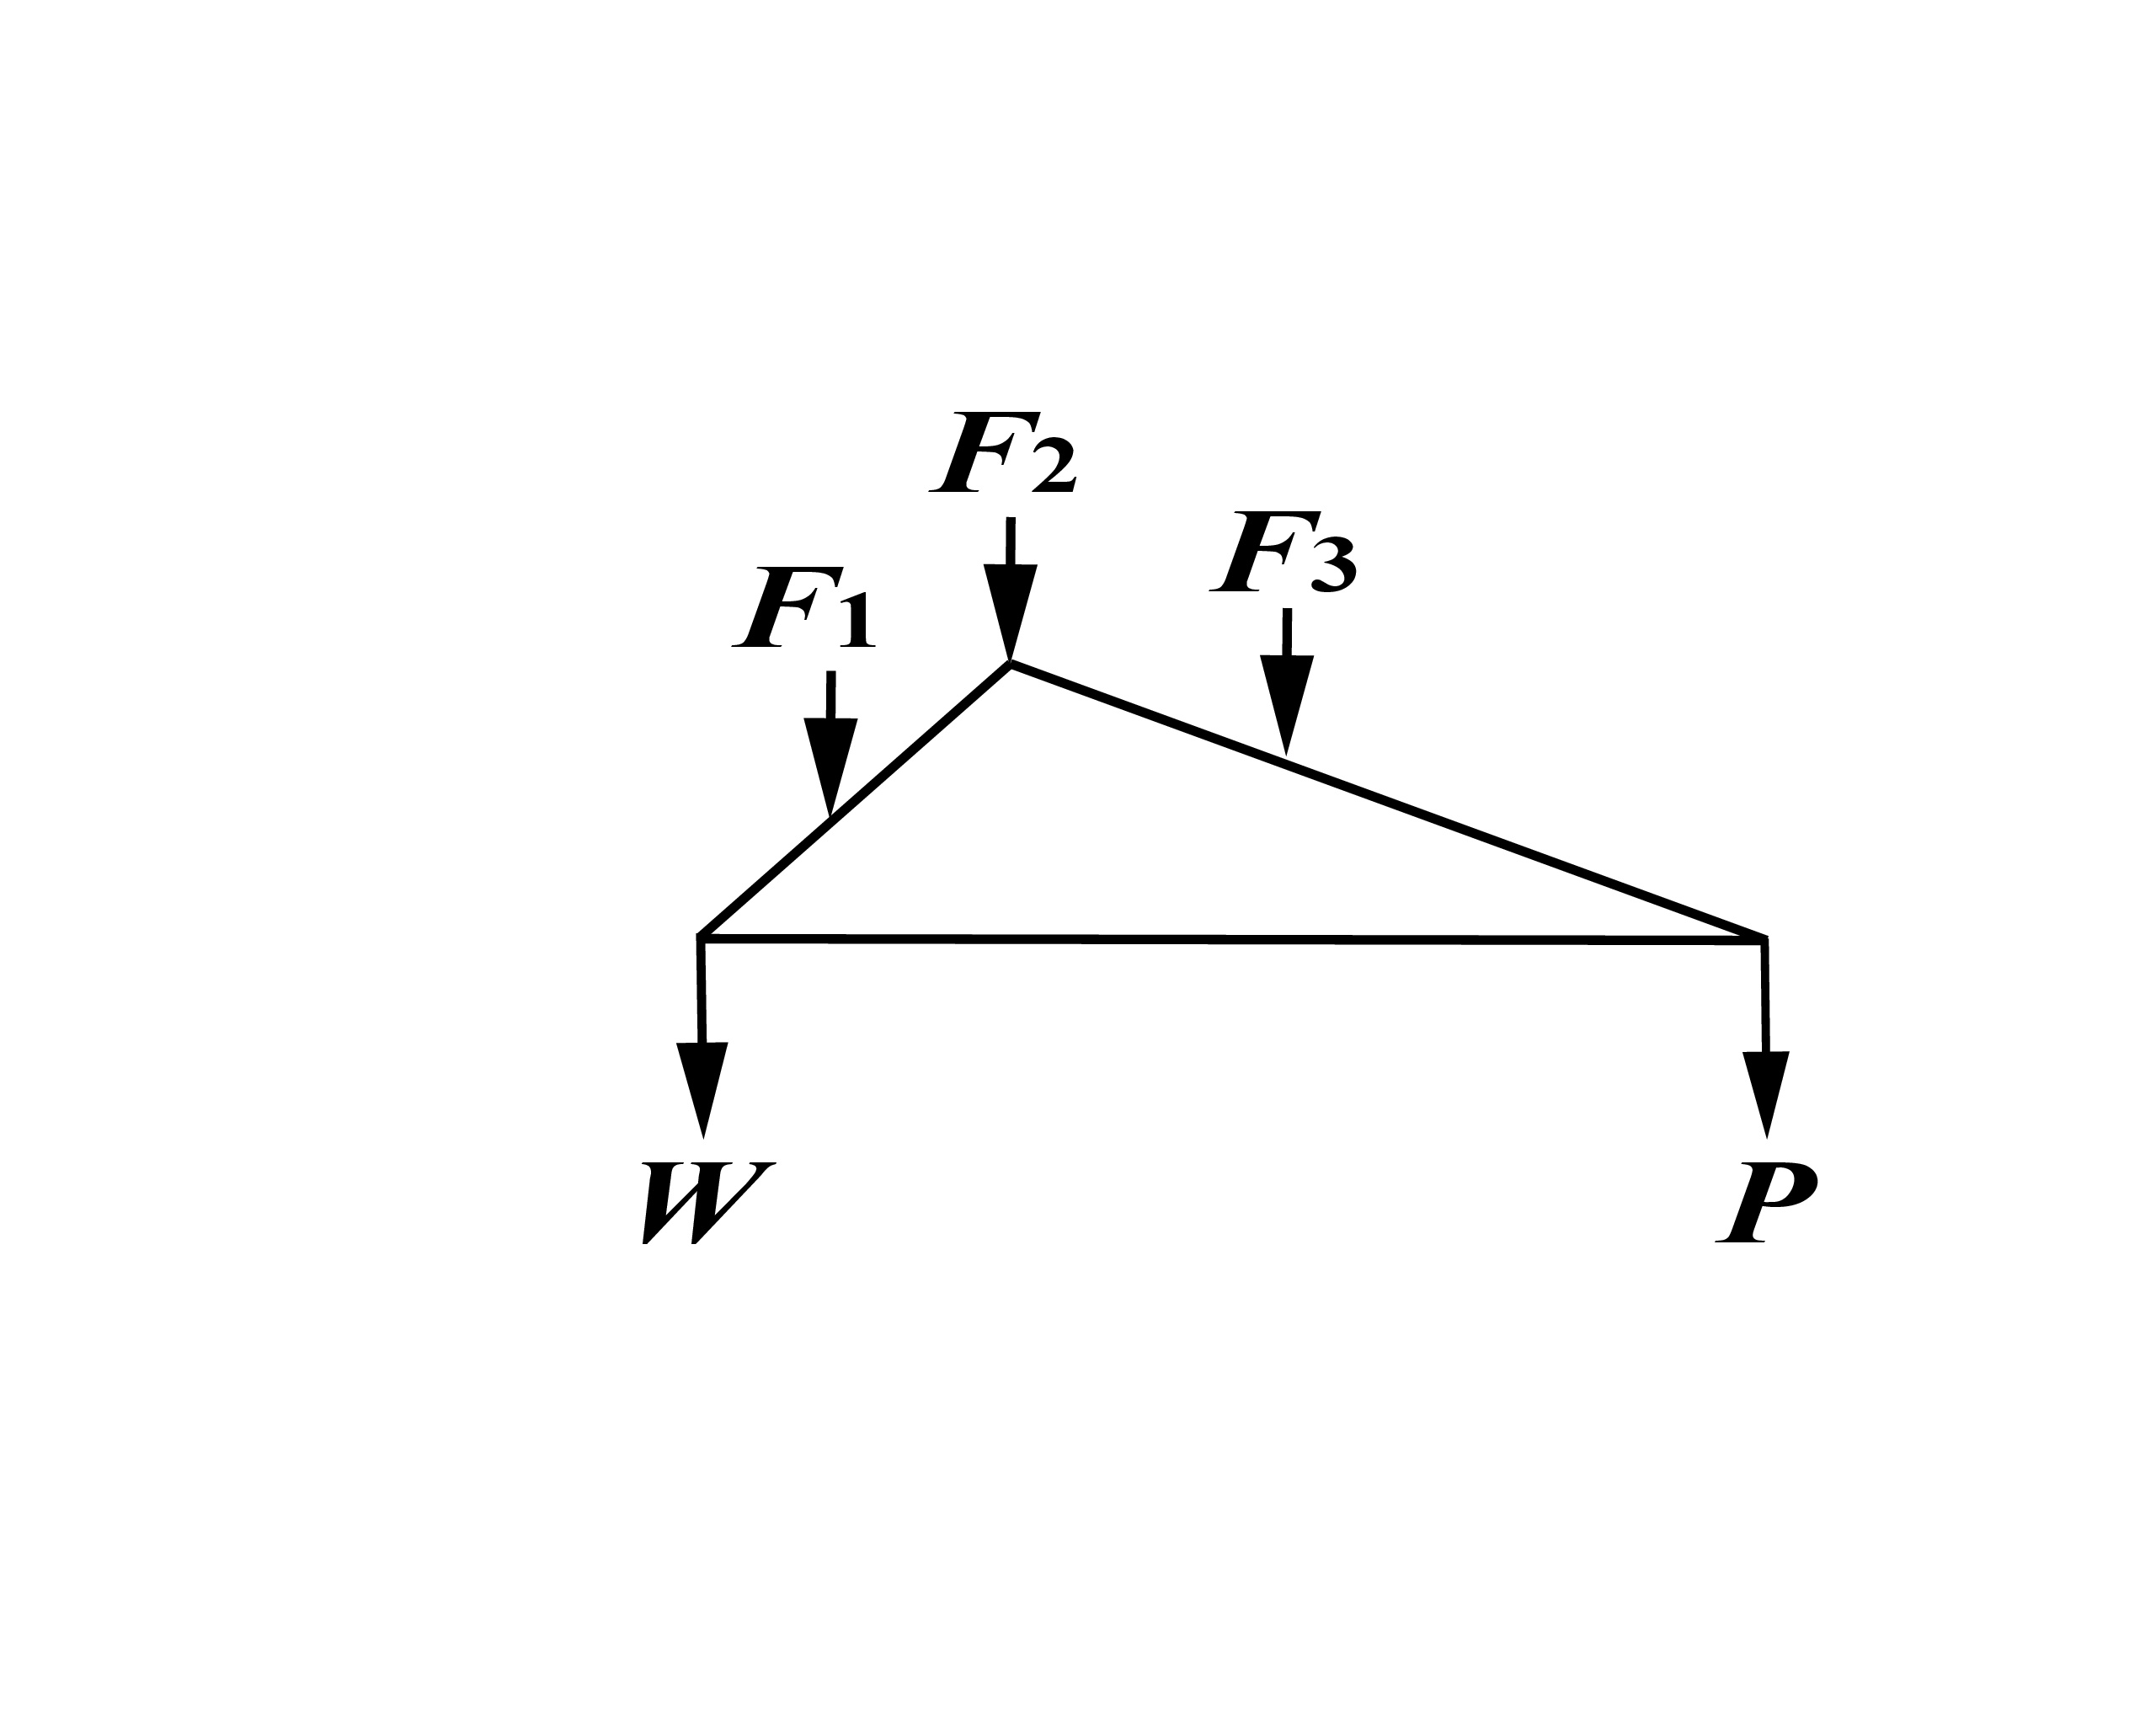
\includegraphics[scale=0.17]{cascades/3in}}
  \caption{Каскад с тремя потоками питания}\label{fig:3_inputs}
\end{figure}

Основным преимуществом использования каскада рис. \ref{fig:3_inputs} является возможность б'ольшей экономии природного урана.
В \cite{smirnovApplyingEnrichmentCapacities2018}, например, демонстрируется экономия половины природного урана на каждом рецикле.
Однако этот эффект достигается ценой дополнительного расхода РР. При этом возможен выбор соотношения разбавителей и, что позволяет регулировать экономию природного урана и перерасход РР.
Эта особенность позволяет «настраивать» каскад для достижения компромисса между этими показателями, которые являются основными (интегральными) характеристиками разделительного процесса.
Такой прием может позволить добиваться оптимального по себестоимости баланса затрат на эти два конкурирующих показателя.
Заметим, что в качестве критериев для выбора оптимальной схемы как правило и используют минимизацию работы разделения и расхода природного урана для получения единицы товарного НОУ. Эти характеристики являются ключевыми для экономики производства низкообогащенного урана. Иными словами, именно они, в основном, и определяют величину удельных затрат на получение коммерческого продукта.

Кроме этого, вариант рис. \ref{fig:3_inputs} полезен для решения проблемы утилизации накопленных объемов обедненного урана \cite{smirnovEnrichmentRegeneratedUranium2014}. Поскольку гексафторид урана является агрессивным веществом, его хранение связано с затратами, и емкости для хранения следует время от времени заменять из-за коррозионных процессов \cite{fitchOPTIONSDISPOSALREAPPLICATION2009, oecdManagementDepletedUranium2001}.

Однако следует отметить, что этот подход предполагает снижение содержания $^{235}$U в образовавшемся ОГФУ, по сравнению с исходным, и требует исследования перспектив дальнейшего использования такого материала в бланкетах реакторах-бридерах.
Произведенный посредством схемы рис. \ref{fig:3_inputs} дважды обедненный ОГФУ, к тому же содержащий повышенную концентрацию минорных изотопов, по-видимому, должен быть первым на очереди к переводу в стабильную форму. Такая переработка, заключающаяся в обеcфторивании и переводе в закись-окись урана, осуществляется на установках типа «W-ЭХЗ» \cite{PererabotkaOGFUObrazovaniem2014}.

Итак, исходя из результатов работы \cite{smirnovApplyingEnrichmentCapacities2018}, схема (рис. \ref{fig:3_inputs}), как и схема рис. \ref{fig:2_inputs}, позволяет обеспечить полный возврат урана в ядерный топливный цикл только для двух первых циклов повторного обращения.
При заданных в работе \cite{smirnovApplyingEnrichmentCapacities2018} условиях, это невозможно для серии последовательных циклов из-за быстрого накопления четных четных изотопов. При  этом отсутствует возможность с помощью такой схемы очистить смеси от этих нежелательных компонентов \cite{smirnovApplyingEnrichmentCapacities2018}.

Таким образом, возникает проблема очистки изотопных составов от четных изотопов, которые имеют тенденцию накапливаться от рецикла к рециклу, приводя к деградации изотопного состава.
Важность сдерживания накопления $^{232}$U при многократном переиспользовании была показана в работе \cite{smirnovEvolutionIsotopicComposition2012}.
Введение ограничения на $^{232}$U позволяет замедлить рост концентрации $^{236}$U в изотопном составе рециклируемого топлива.

Однако, как было отмечено, во всех рассмотренных схемах заметное снижение содержания изотопов $^{232,234,236}$U в финальном НОУ достигается, прежде всего, за счет разбавления регенерата внутри каскада смесями, полученными из урана природного состава (НОУ, ОГФУ, или сам природный уран).

Отсюда возникает вопрос отделения четных $^{232,234,236}$U из изотопного состава рециклируемого материала.

В качестве дополнительного аргумента для поиска альтернативных каскадов, позволяющих выводить из системы $^{232,234,236}$U, приведем следующий факт.
В последнее время конструкция ВВЭР развивалась к увеличению максимального выгорания топлива (до 70 МВт-день / кг U в ВВЭР-1200) \cite{asmolovNewGenerationFirstofthe2017}, с целью снижения стоимости топливной составляющей \cite{andrianovaPovyshenievygoraniyaToplivaVVER2008}.
Имея ввиду, что, согласно природе цепной реакции, рост остаточного содержания $^{232,234,236}$U пропорционален уровню выгорания \cite{VeryHighBurnups2006}, схемы, нацеленные на очистку $^{232,234,236}$U заслуживают особого внимания.

К тому же, в случае успеха в продвижении российских услуг по реконверсии RepU на мировом рынке, очистка от $^{232}$U может быть востребована в силу ограничения лицензии российского оператора ($5\cdot10^{-7}$\% (5ppb) по $^{232}$U), если не будут применены иные способы улучшения изотопного состава.
Однако существуют практики возврата регенерата в ЯТЦ, для которых проблема очистки регенерата от четных $^{232,234}$U не актуальна вне необходимости многократного рецикла. Так, Французская электроэнергетическая компания EDF выбрала стратегию прямого обогащения регенерированного урана. Такой подход воплощен на АЭС Cruas, которая имеет лицензию на работу с топливом, в котором ограничение содержания $^{232}$U в 6 раз выше ограничения, принятого в РФ, и составляет 30 ppb.

Итак, далее будут представлены способы, с помощью которых можно частично удалить нежелательные изотопы из системы.

Это может быть сделано с помощью схем, которые позволяют извлекать промежуточный продукт, или с помощью составных схемам (несколько последовательных каскадов, например, двойной каскад).
Перейдем к рассмотрению первых.

\subsubsection{Применение дополнительных потоков отбора}
Схемы, называемые каскадами с промежуточным продуктом были предложены с целью «очистки» от четных изотопов параллельно с производством основного НОУ-продукта (рис. \ref{fig:3_out}) \cite{zhurinSPOSOBPERERABOTKIZAGRYaZNENNOGO, palkinAnaliticheskiyRaschetSoderzhaniya2007}.
Здесь в качестве основного продукта получают НОУ требуемых характеристик, а в качестве промежуточного продукта получают состав с пониженным содержанием нежелательных изотопов.
\begin{figure}[ht]
  \centerfloat{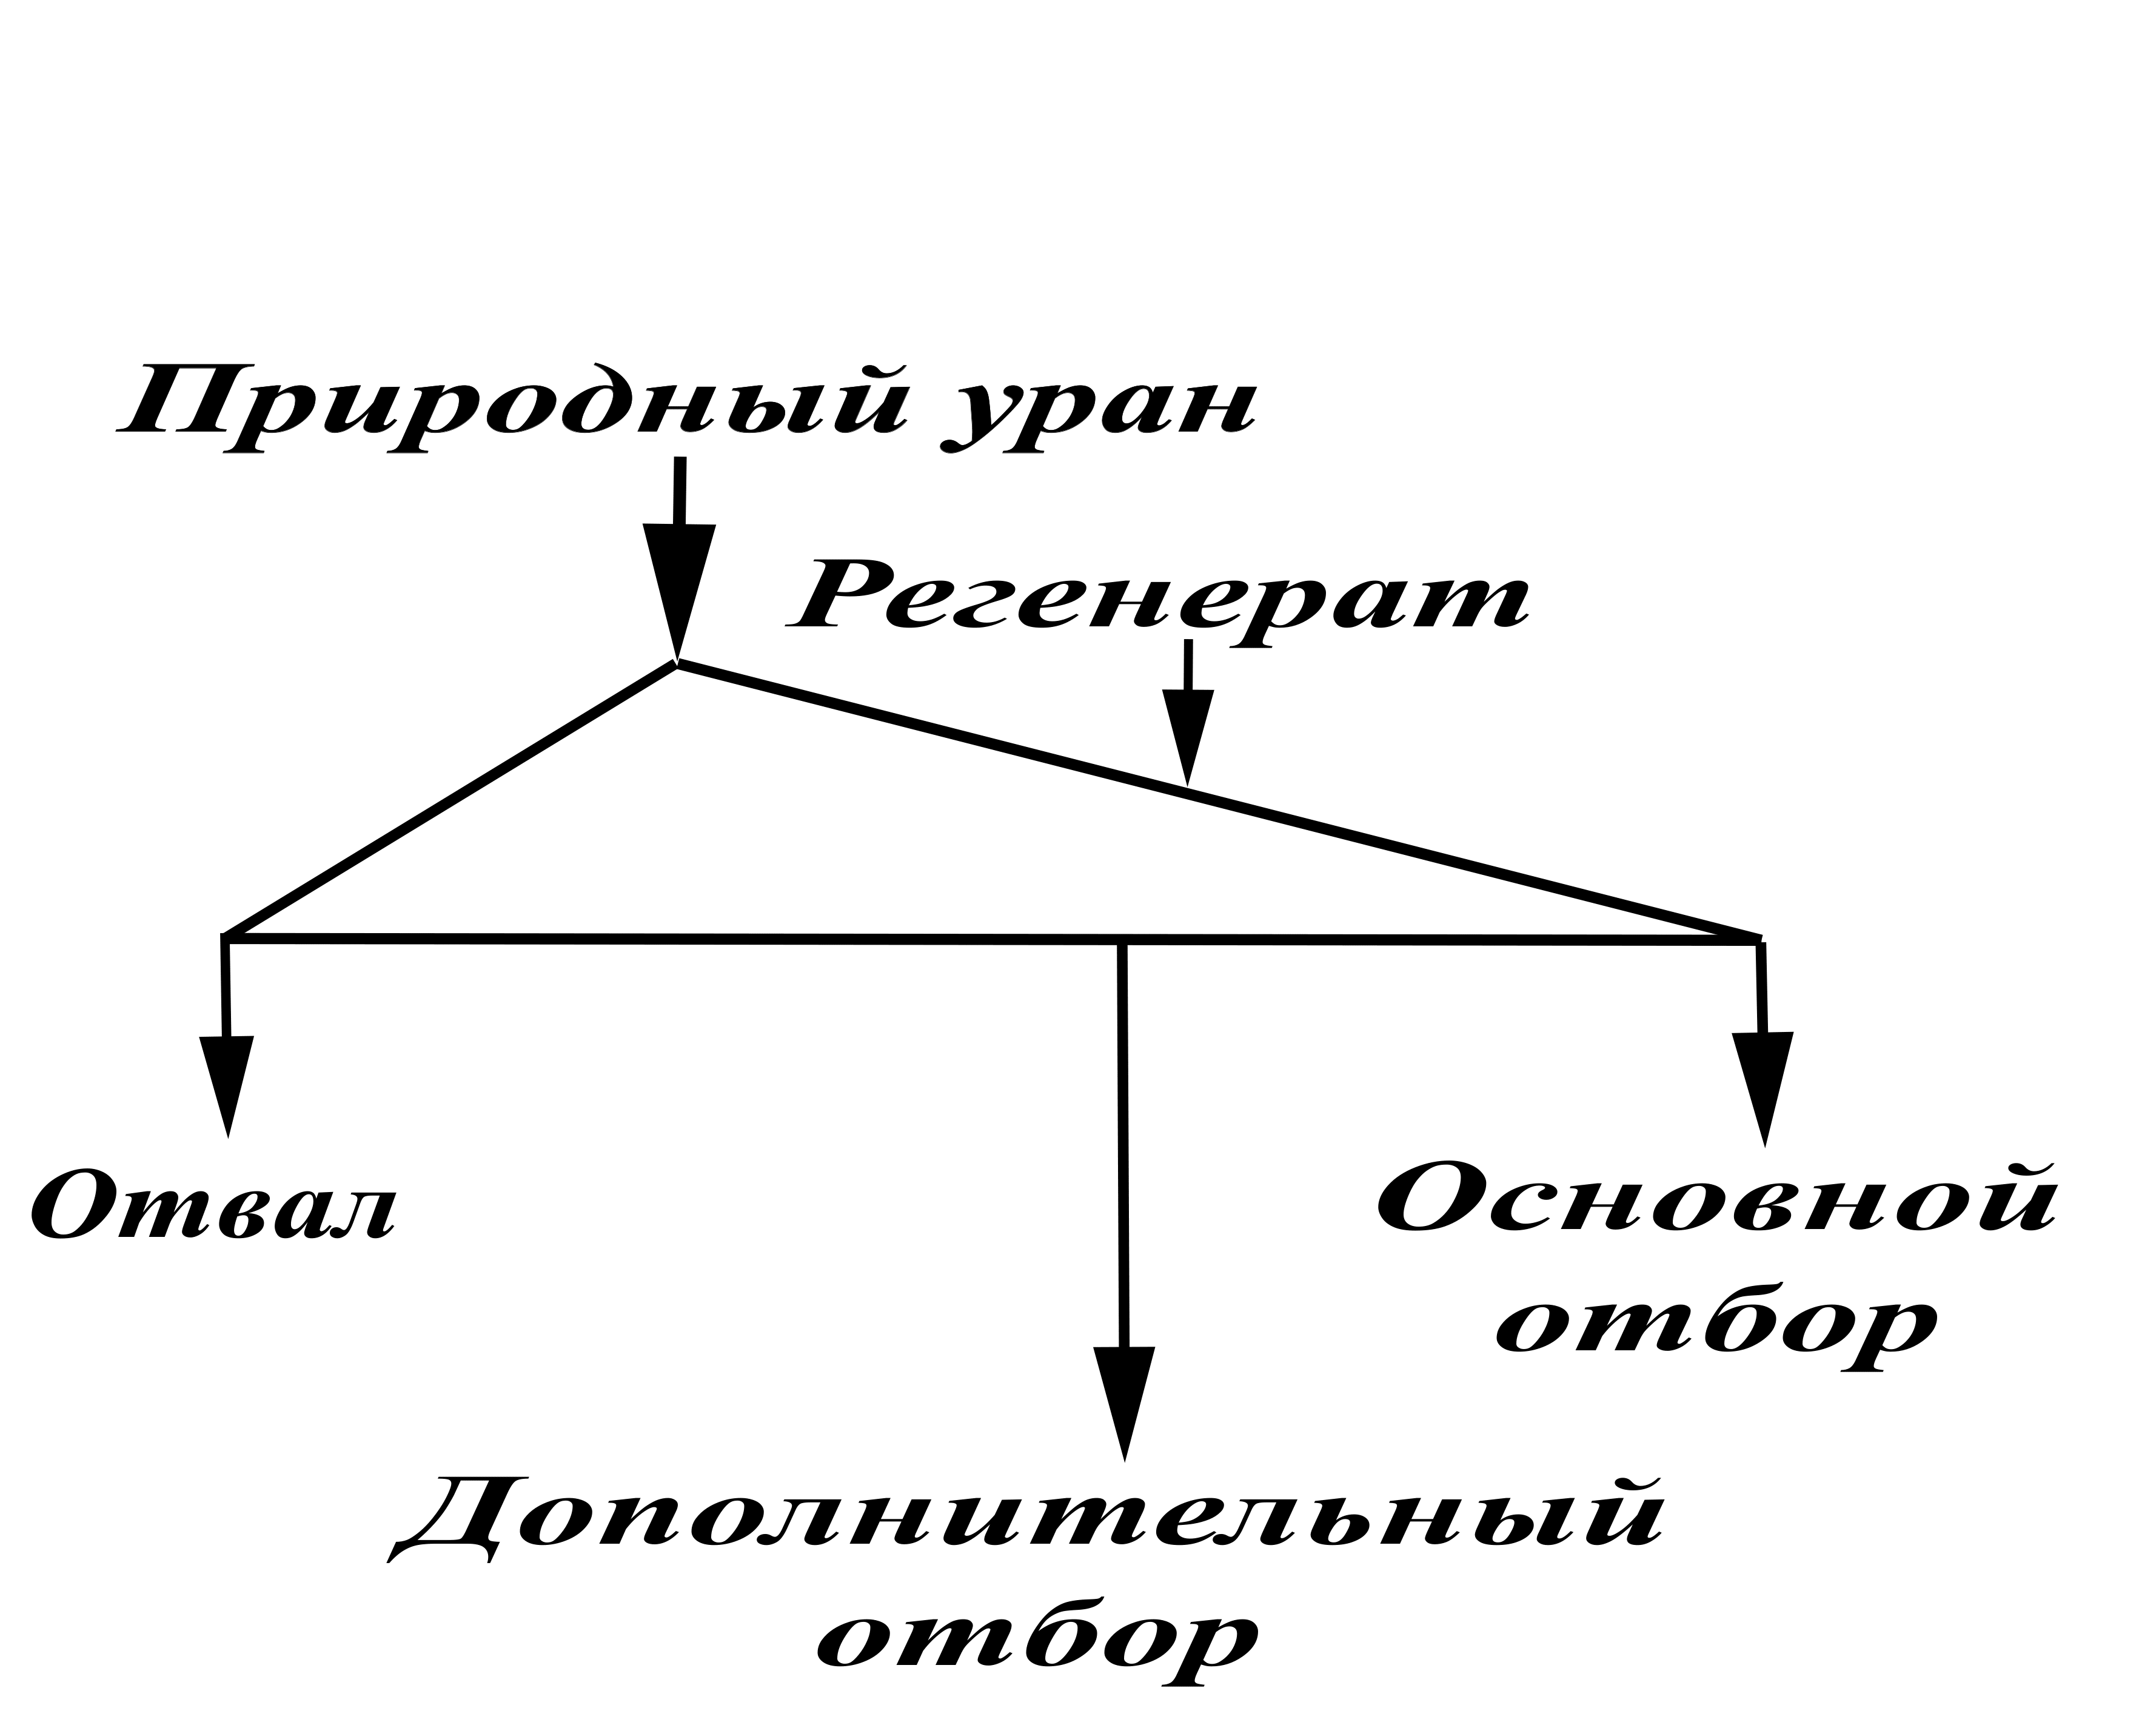
\includegraphics[scale=0.07]{cascades/3out}}
  \caption{Каскад с дополнительным потоком отбора}\label{fig:3_out}
\end{figure}

Частичное удаление из смеси четных изотопов на первой стадии, позволяет получить больше преимуществ от увеличения количества делящегося $^{235}$U на второй -- при ее обогащении до товарного НОУ \cite{palkinSeparationUraniumIsotopes2010}.

Концентрация $^{235}$U в этом "очищенном" продукте подбирается так, чтобы она минимально отличалась от концентрации в потоке дополнительного питания в виде регенерата.
Это позволяет при соблюдении эквивалентности этих потоков исключить потери работы разделения.
Как показано в \cite{palkinSeparationUraniumIsotopes2010}, в результате очистки содержание всех четных изотопов значительно снижается. После чего, низкообогащенный уран с концентрациями $^{232,234,236}$U, удовлетворяющими требования ASTM для коммерческого продукта, может быть получен из очищенного промежуточного продукта путем его прямого обогащения \cite{shopenSposobPolucheniyaRazbavitelya2008}.
При этом важно заметить, что основной продукт НОУ каскада-очистителя также соответствует этим требованиям \cite{palkinSeparationUraniumIsotopes2010}. Следует отметить, что высокое качество очищенного регенерата достигается только при малой доле потока регенерата, относительно природного урана, в случае, когда необходимо выполнить требования к каждому из производимых НОУ.
Основным преимуществом здесь является то, что эта схема, обеспечивающая одновременное снижение $^{232,234,236}$U, практически не теряет РР и не требует загрязнения дополнительного каскада (будет обсуждаться далее в разделе составных схем).

Однако, важно отметить, что ввиду необходимости использовать в несколько раз большую доли природного урана в питании, этот каскад является по существу схемой разбавления регенерата.

Недостатки здесь заключаются в том, что эффект очистки обусловлен, прежде всего, уменьшением объема потока очищенного промежуточного продукта. Эффекта заметного снижения содержания минорных изотопов в дополнительном отборе можно добиться лишь при сильном разбавлении регенерата природным сырьем, в соотношениях, лежащих в диапазоне (1-25)/100 \cite{palkinSeparationUraniumIsotopes2010, smirnovKaskadnyeShemyZadachah2012}.
Следовательно, данная схема не может обеспечить широкомасштабного возврата регенерированного урана в топливный цикл ВВЭР, ввиду малой удельной экономии природного урана.
Более того, такой подход демонстрирует снижение экономии природного урана.

В качестве материалов, которые необходимо очистить посредством такой схемы, можно рассматривать составы загрязненного урана природного состава, «хвостов» процесса обогащения и других, «загрязненных» урановыми $^{232,234,236}$U \cite{palkinSeparationUraniumIsotopes2010}. 

Таким образом, задача возврата регенерата в ЯТЦ в виде низкообогащенного урана требует дальнейших поисков эффективных схем, так как предложенный каскад рис. \ref{fig:3_out} демонстрирует снижение экономии природного урана, и не позволяет вернуть весь ОЯТ (в соотношении к продукту 1:1).

Рассмотрев схему, которая позволяет извлекать промежуточный продукт, перейдем к обзору многокаскадных схем.


\subsection{Комбинации нескольких каскадов (составные схемы)}\label{sec:ch1/sec2.3}
Под составными схемами подразумеваются различные вариации коммутации одиночных каскадов в единую составную схему.

\subsubsection{Двойной каскад}

Рассмотрим принципы работы простейшего варианта составного каскада -- двойного каскада (рис. \ref{fig:double_ru}).
Эта модификация направлена на эффективное удаление $^{232}$U из каскада и нацелена на получение НОУ реакторного качества без необходимости вовлечения природного урана \cite{SosninYuChelcov, TehnicheskieResheniyaPo}.
Рассмотрим принципы работы такой схемы.
В первом каскаде (верхнем) $^{235}$U обогащается по легкой фракции (отбор первого каскада на рис. \ref{fig:double_ru}), где также накапливается $^{232}$U.
Затем, эту смесь направляют во второй каскад, где самые легкие изотопы $^{232,234}$U концентрируется в загрязненной "отборной" части и выводится из обращения.
В то же время НОУ-продукт с требуемым уровнем обогащения по $^{235}$U направляется с тяжелой фракцией к другому выходу, в этой конфигурации представляющим из себя поток продукта.
\begin{figure}[ht]
  \centerfloat{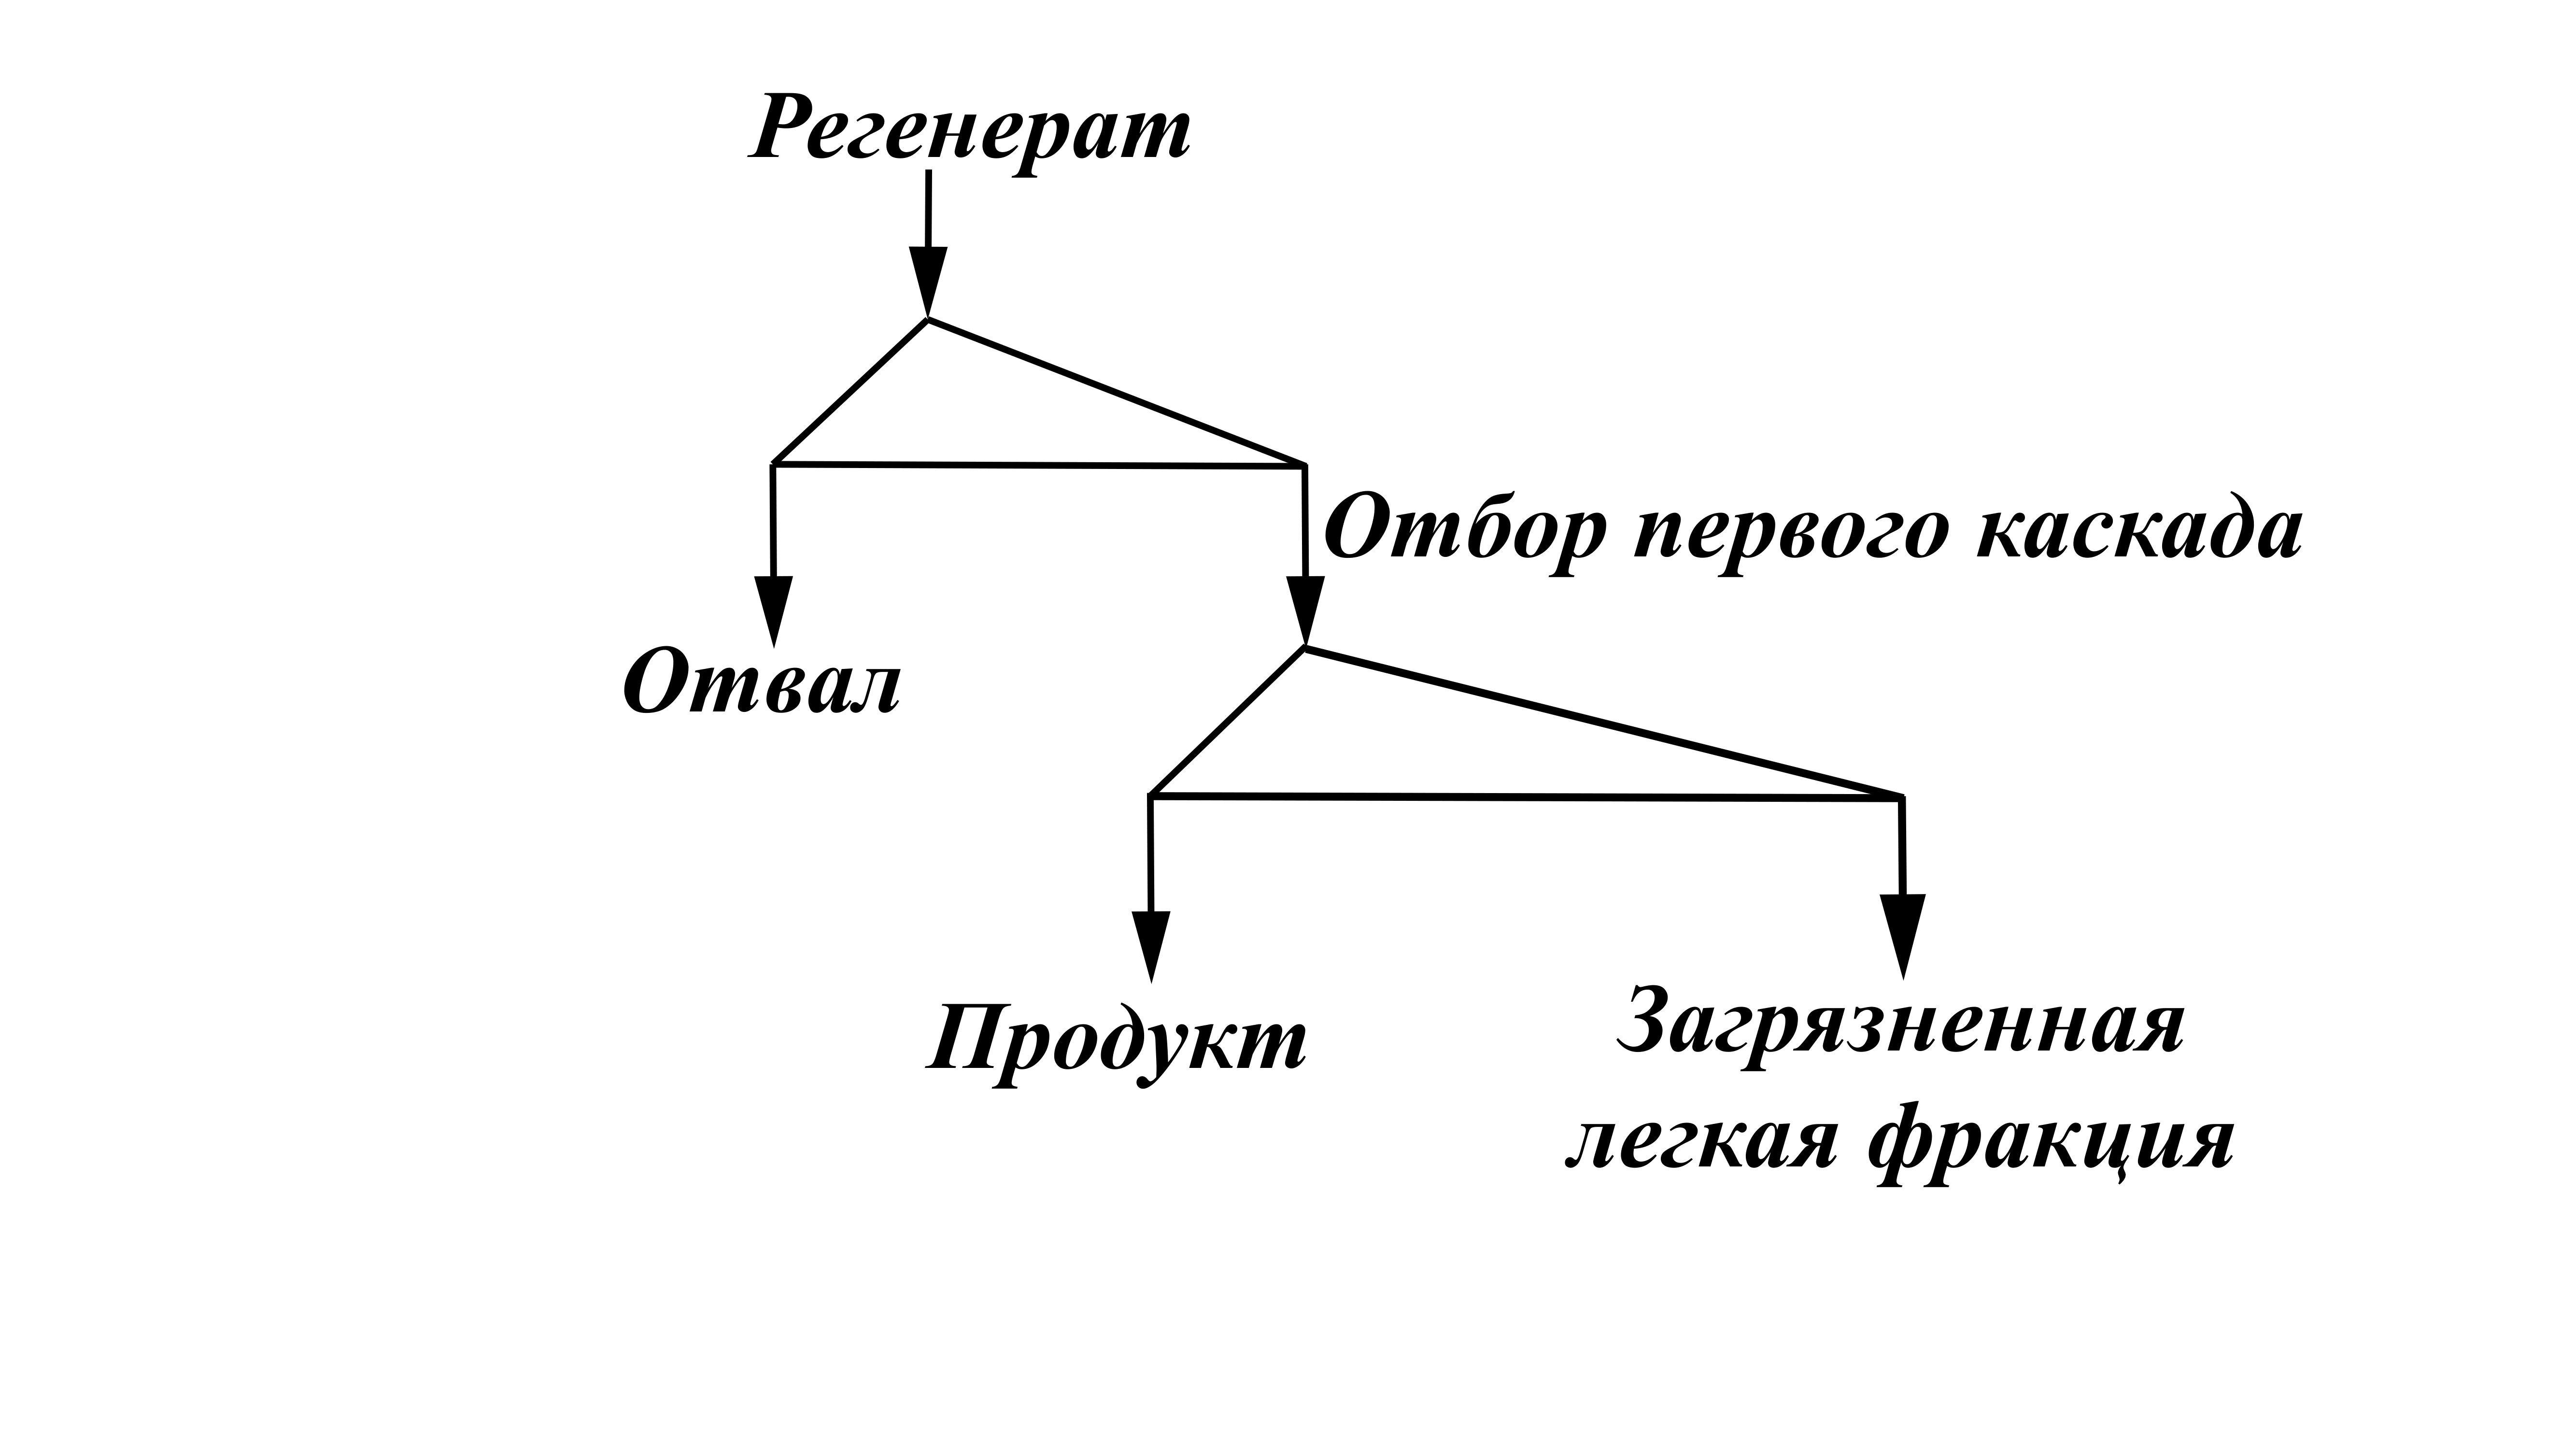
\includegraphics[scale=0.07]{cascades/double_ru}}
  \caption{Двойной каскад}\label{fig:double_ru}
\end{figure}

Рассмотрим физический эффект, который происходит в легком конце второго каскада, на котором необходимо сконцентрировать четные изотопы.
При доведении концентрации $^{235}$U до уровня, свойственного оружейному материалу, наблюдается разворот кривой монотонно возрастающей концентрации $^{235}$U, тогда как прекращение обогащения смеси по $^{232,234}$U (а также $^{233}$U, который учитывается не во всех рассмотрениях) не происходит.

Таким образом, с помощью этого приема во втором каскаде осуществляется пространственное разделение легкой фракции с $^{232,233,234,235,236}$U и тяжелой с $^{235,236,238}$U.
Как результат, возможность удалять из изотопной смеси легкие четные изотопы связана с потерями ценного $^{235}$U в выводимом потоке.
К тому же, такой материал классифицируется как высокообогащенный уран.
А так как материал такой категории считается крайне ценным, возникает вопрос о целесообразности его окончательной утилизации.
Более того, загрязненность этой фракции $^{232}$U, требует особых условий обращения, а ее утилизация может быть крайне дорогостоящей операцией.
Эти два фактора ставят проблему обращения с легкой фракцией второго каскада, пути решения которой будут описаны в последующих разделах.

В качестве примера реализации такой схемы, в \cite{vodolazskihSposobIzotopnogoVosstanovleniya} предлагается обогащать изотопную смесь регенерата до уровня оружейного (> 90\% $^{235}$U) уже в первом ординарном каскаде.
Это позволяет в тяжелой фракции второго каскада добиваться содержания $^{232}$U на уровне сырьевого регенерата.

В некоторых случаях схема рис. \ref{fig:double_ru}) подразумевает использование газа-носителя (или буферного газа) \cite{prusakovCorrectingIsotopicComposition2008, SposobIzotopnogoVosstanovleniyab}.
В качестве такого газа-носителя используется буферное газообразного соединения, которое является инертным (неактивным) к гексафториду урана -- рабочему газу. 
Это позволяет повысить эффективность отделения $^{232}$U от регенерированного урана и уменьшить потери $^{235}$U.
Идея применения этого газа с массовым числом, близким к $^{232}UF_6$, была выдвинута в \cite{SosninYuChelcov}, исходя из предположения, что такой газ мог бы служить матрицей-носителем для $^{232}UF_6$.
В этом исследовании авторы предложили использовать фреон-346 $C_{8}H_{3}F_{13}$, поскольку среднее массовое количество этого соединения практически совпадает с массовым числом $^{232}UF_6$ (и ниже, чем в $^{235}UF_6$, что немаловажно).
К тому же, $C_{8}H_{3}F_{13}$ является инертным по отношению к гексафториду урана и не вступает в реакцию с материалами газовой центрифуги, однако требует проведения операции разделения в ограниченном интервале давлений, создаваемых центробежным полем газовой центрифуги \cite{prusakovCorrectingIsotopicComposition2008}.

Оба рассматриваемых варианта -- с газом-носителем, и без -- разделяют следующие недостатки:
\begin{enumerate}
  \item оба каскада в схеме загрязнены изотопом $^{232}$U, что осложняет радиационную обстановку на разделительном производстве.
  \item в предлагаемой схеме принципиально отсутствует возможность снижения накопления изотопа $^{236}$U, негативное влияние которого на размножающие характеристики тепловыделяющих сборок (ТВС) требует дополнительного обогащения по изотопу $^{235}$U. При этом эквивалентная концентрация $^{235}$U может быть заметно больше, чем в штатном топливе, что обуславливает дополнительные затраты работы разделения.
\end{enumerate}

При этом вариант с газом-носителем, требует очистки получаемого товарного продукта от этого газа, что, очевидно, также приводит к увеличению удельных затрат.

Отсюда, поскольку в ходе технологического процесса не возникает необходимости очищать смесь от буферного газа, вариант без этого газа более предпочтителен, \cite{smirnovKaskadnyeShemyZadachah2012}.

Среди недостатков рассматриваемых схем следует также отметить следующее.
Некоторые конфигурации предполагают получение высокообогащенного урана с содержанием $^{235}$U более 20\%, что усложняет проблему соответствия международным стандартам обращения с делящимися материалами.
Так, в \cite{palkinPurificationReprocessedUranium2016} подчеркивается, что, тогда как в первом же каскаде достигается концентрация >20\% от $^{235}$U, которая затем во втором каскаде еще больше повышается в потоке, уносящем "загрязненную" фракцию, такая мера едва ли будет одобрена ввиду строгих ограничений на производство ВОУ во всем мире \cite{ManagementHighEnriched2005}.

Также существует вариант реализации двойного каскада, в котором исключаются высокие концентрации $^{235}$U \cite{zhurinSposobIzotopnogoVosstanovleniya2010}.
В таком исполнении, принцип работы несколько меняется.
В этом каскаде гексафторид восстановленного по изотопному составу урана нарабатывают в потоке отбора второго каскада.
Иллюстрация такой схемы представлена на рис. \ref{fig:pure_double}.

\begin{figure}[ht]
  \centerfloat{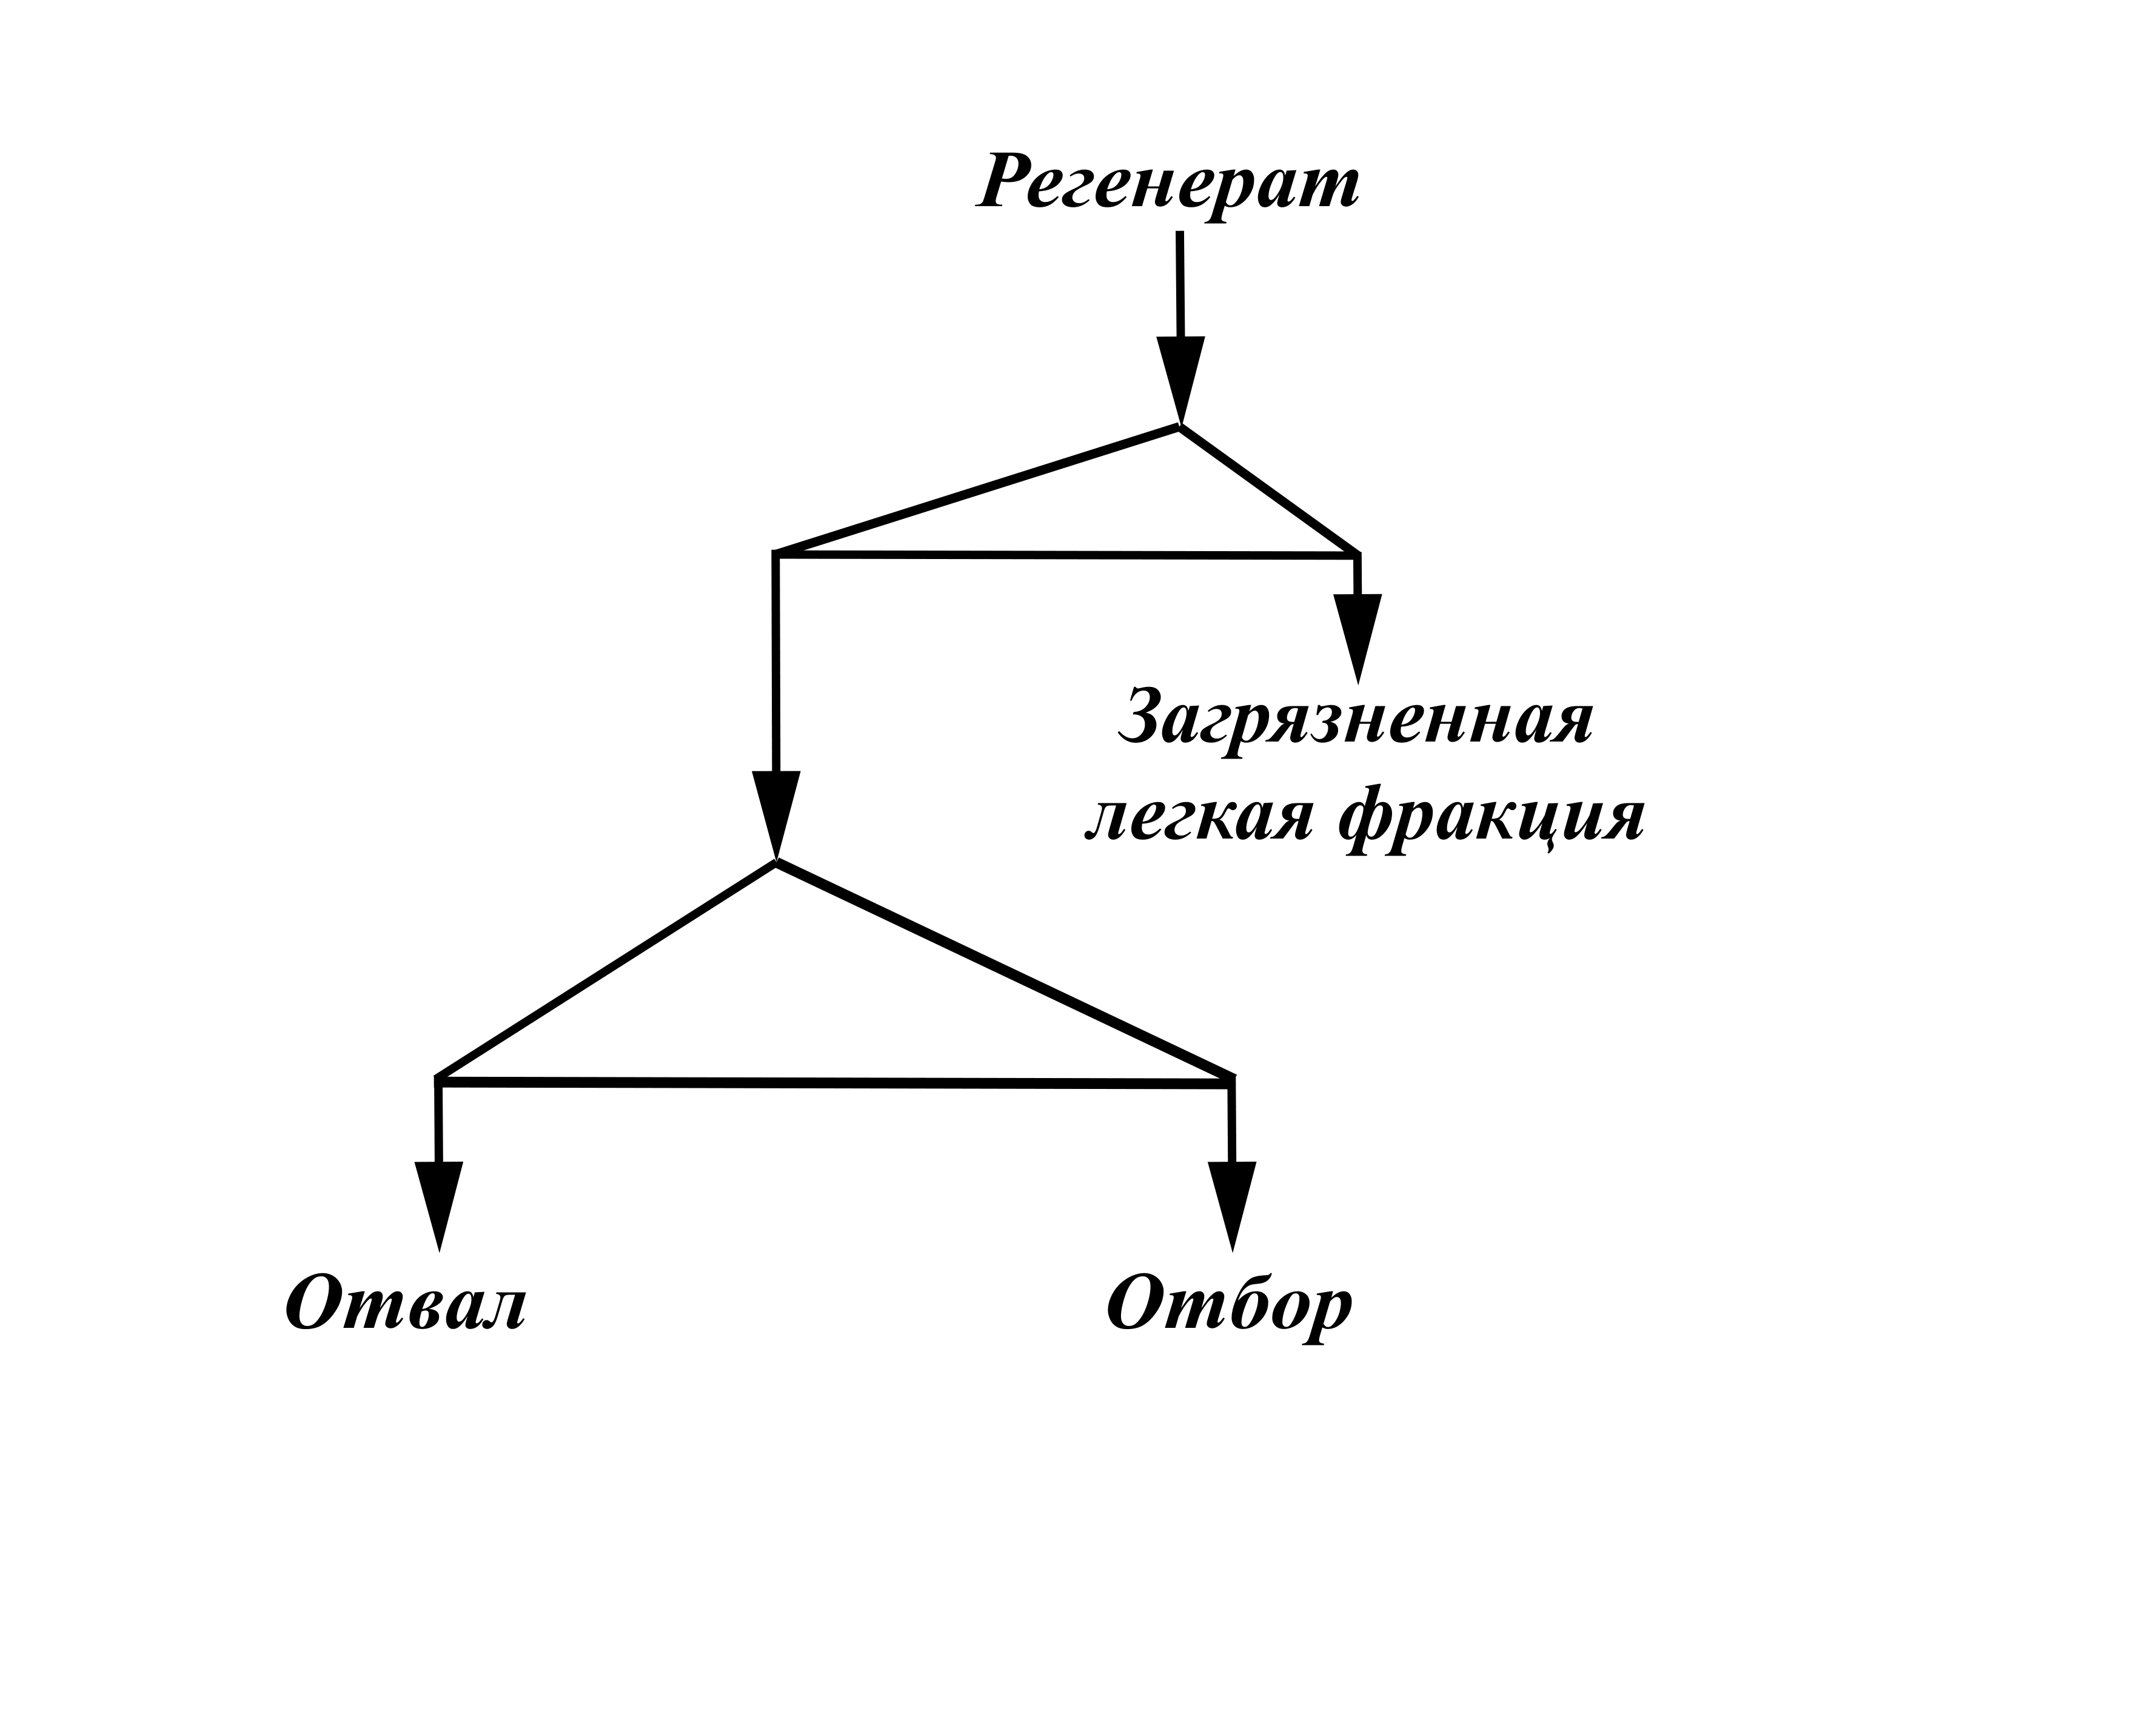
\includegraphics[scale=0.1]{cascades/pure_double}}
  \caption{Двойной каскад с очисткой в первом каскаде}\label{fig:pure_double}
\end{figure}

Здесь второй каскад запитывается тяжелой фракцией первого каскада, полученной при обогащении легкой фракции первого каскада изотопом $^{235}$U до концентрации,не превышающей 20\%.
В такой варианте схемы двойного каскада роль каскада, на котором производится очистка от легких четных изотопов, принимает первый ординарный каскад.

Как подвид такой схемы в работе \cite{palkinReprocessedUraniumPurification2013} предлагается использовать прием смещения точки подачи питания в сторону точки отбора легкой фракции первого каскада.
При этом отмечается, что это позволяет добиться существенного снижения доли $^{232}$U в конечном продукте, а также, при высокой степени обогащения в первом каскаде, уменьшения содержания $^{234,236}$U.
Однако, такой вариант связан с существенными потерями работы разделения и не позволяет осуществлять эффективную очистку от $^{234,236}$U \cite{palkinPurificationReprocessedUranium2016}.

В главе 3 будет приведен расчетный анализ для выявления физических закономерностей, позволяющих судить о пригодности таких схем для задачи обогащения регенерата в условиях многократного рецикла.

Итак, двойной каскад имеет уникальное преимущество, которое состоит в возможности повторно обогащать регенерированный уран, даже не разбавляя его иным дополнительным сырьем, которым, как правило, выступает природный уран или его производные.
Это свойство делает двойной каскад наилучшим вариантом с точки зрения экономии природного урана.
Однако оно не предотвращает существенных потерь $^{235}$U из топливного цикла, которые связаны с образованием незадействованного потока, призванного извлечь нежелательные $^{232,234}$U.
Также у схемы существует недостаток, если речь идет о поставленной задаче производства НОУ из эквивалентного количества ОЯТ, если при этом требуется гомогенное топливо.
Тогда приходится иметь дело с неспособностью двойного каскада обеспечить заданной пропорции (1:1) возврата регенерированного материала в ядерный топливный цикл.
Такой каскад расходует значительно больше необходимого $\approx$0,93 кг регенерата на производство 1 кг свежего НОУ.
Это означает, что для загрузки реактора, в котором используется переработанное топливо, необходимо будет использовать другой источник, например, природный уран, в отдельных тепловыделяющих элементах (ТВЭЛах) или целых ТВС. 
Как результат, в контексте замыкания ЯТЦ по урановой составляющей и возврата в рассматриваемый реактор всего объема топлива, реальная экономия природного урана будет не 100\%, а в несколько раз меньше -- в лучшем случае 15-20\%.

Таким образом, для преодоления недостатка двойного каскада, связанного с невозможностью добиться желаемого соотношения финального продукта и питающего регенерата, необходима его модификация.
Такая модификация, предложенная в работе \cite{smirnovObogashchenieRegenerirovannogoUrana2018}
будет рассмотрена в основной части диссертационной работы (в третьей главе).
Далее продолжим детальное рассмотрение иных возможных комбинаций каскадов.

\subsubsection{Другие варианты реализации}
Рассмотрим другие способы коммутации каскадов в составные схемы из различных видов одиночных каскадов.

В работе \cite{palkinPurificationReprocessedUranium2016}, представившей схему рис. \ref{fig:int_double}, принцип работы каскада состоит в следующем.

\begin{figure}[ht]
  \centerfloat{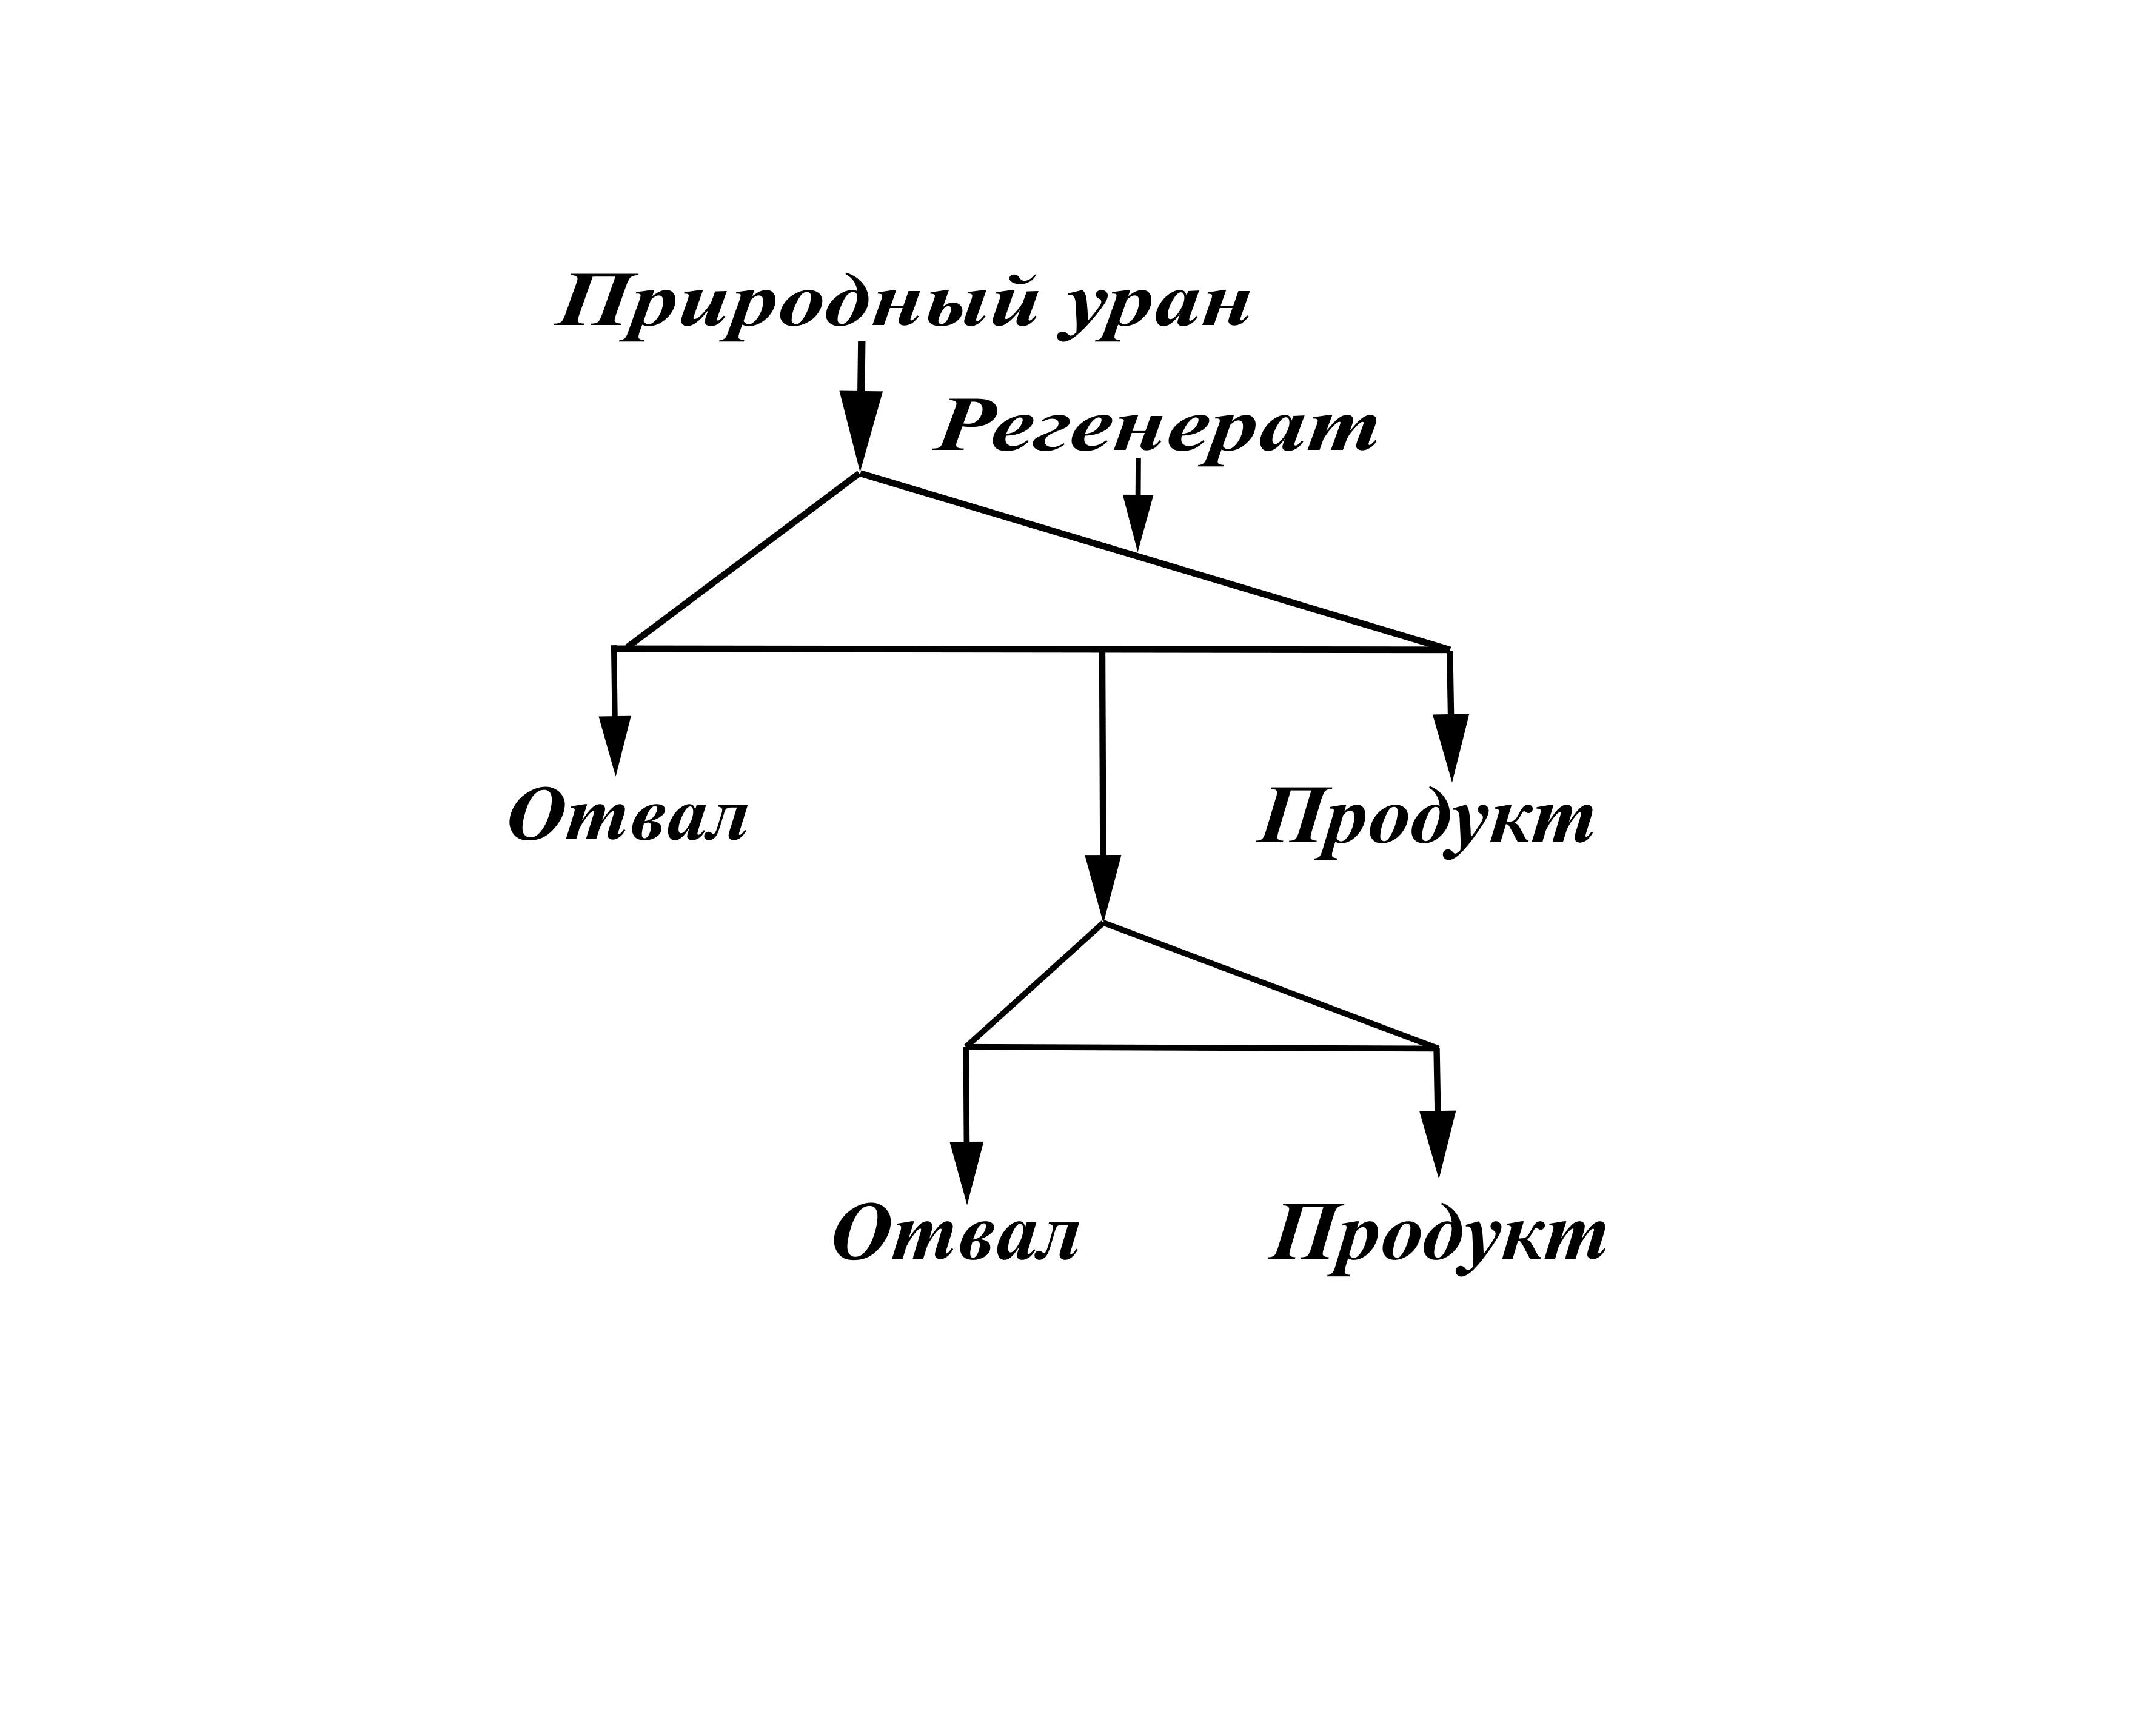
\includegraphics[scale=0.1]{cascades/int_double}}
  \caption{Двойной каскад на основе каскада, получающего очищенный регенерат}\label{fig:int_double}
\end{figure}

В первом в последовательности каскаде в качестве промежуточного продукта -- в дополнительном выходящем потоке в виде очищенного регенерата -- получен изотопный состав с пониженной концентрацией $^{232}$U.
Затем такой очищенный полупродукт поступает в ординарный каскад, как показано на рисунке \ref{fig:int_double}, где он обогащается до необходимого уровня по $^{235}$U.
При этом, основной продукт первого каскада также может соответствовать заданным свойствам коммерческого НОУ.
Вдобавок, автор данной работы подчеркивает возможность значительного снижения нежелательной концентрации $^{236}$U в случае уменьшения потока дополнительного отбора -- промежуточного продукта первого каскада.
Автор рекомендует применять этот эффект следующим образом: например, снизить концентрации  $^{234}$U и  $^{236}$U в промежуточном продукте (16\% для  $^{236}$U), при этом всего лишь слегка уменьшив (всего на 4\%) поток этого полупродукта.
К тому же, увеличение этого выходящего потока "очищенного" продукта приводит к снижению в нем $^{235}$U.

Каскады с дополнительным продуктом также могут послужить для решения задачи наработки разбавителя для ВОУ \cite{palkinPOLUChENIERAZBAVITELYaDLYa2017}, как показано в \cite{shopenSposobPolucheniyaRazbavitelya2008}.
Это дает возможность задействовать наиболее ценный ресурс -- делящийся изотоп $^{235}$U, который преобладает в оружейном уране (> 90\% $^{235}$U).
Следует отметить, что природный уран, содержание $^{235}$U в котором намного меньше, чем в ВОУ, не достаточно пригоден в качестве разбавителя для ВОУ
Это связано с присутствием в природном уране изотопа $^{234}$U -- сильного альфа-излучателя.
Поэтому, в качестве разбавителя необходимо использовать изотопную смесь с пониженным содержанием $^{234}$U.
В качестве такого материала обычно используется предварительно обогащаемый обедненный уран.
Так, в ходе реализации сделки ВОУ-НОУ \cite{korotkevichRealizaciyaProgrammyVOUNOU2003}, использовали наработанный из отвалов разделительного производства обогащенный до 1,5\% разбавитель \cite{SposobPolucheniyaRazbavitelya}.

Рассмотрев дополнительные варианты применения таких схем, вернемся к их приложению к задаче обогащения регенерированного урана.

На рис. \ref{fig:double_palk} первый каскад, питаемый регенератом, концентрирует изотопы $^{232}$U и $^{234}$U на легком конце, тогда как второй каскад дополнительно подпитывается природным ураном.
Такая модификация, как показано в работе , позволяет «глубоко очищать» обработанную смесь от $^{232}$U, $^{234}$U и уменьшать  $^{236}$U, оставаясь в рамках заданных ограничений.
Этого можно достичь с помощью оптимизации концентрации $^{232}$U в продукте, варьируя точку подачи, при этом минимизируя количество газовых центрифуг.
В этом случае, в отвальном конце каскада будет на порядок снижено содержание вредного $^{232}$U.
Эта стадия позволяет подготовить из регенерированного урана изотопный состав с меньшим содержанием $^{232}$U для последующих этапов обогащения.
\begin{figure}[ht]
  \centerfloat{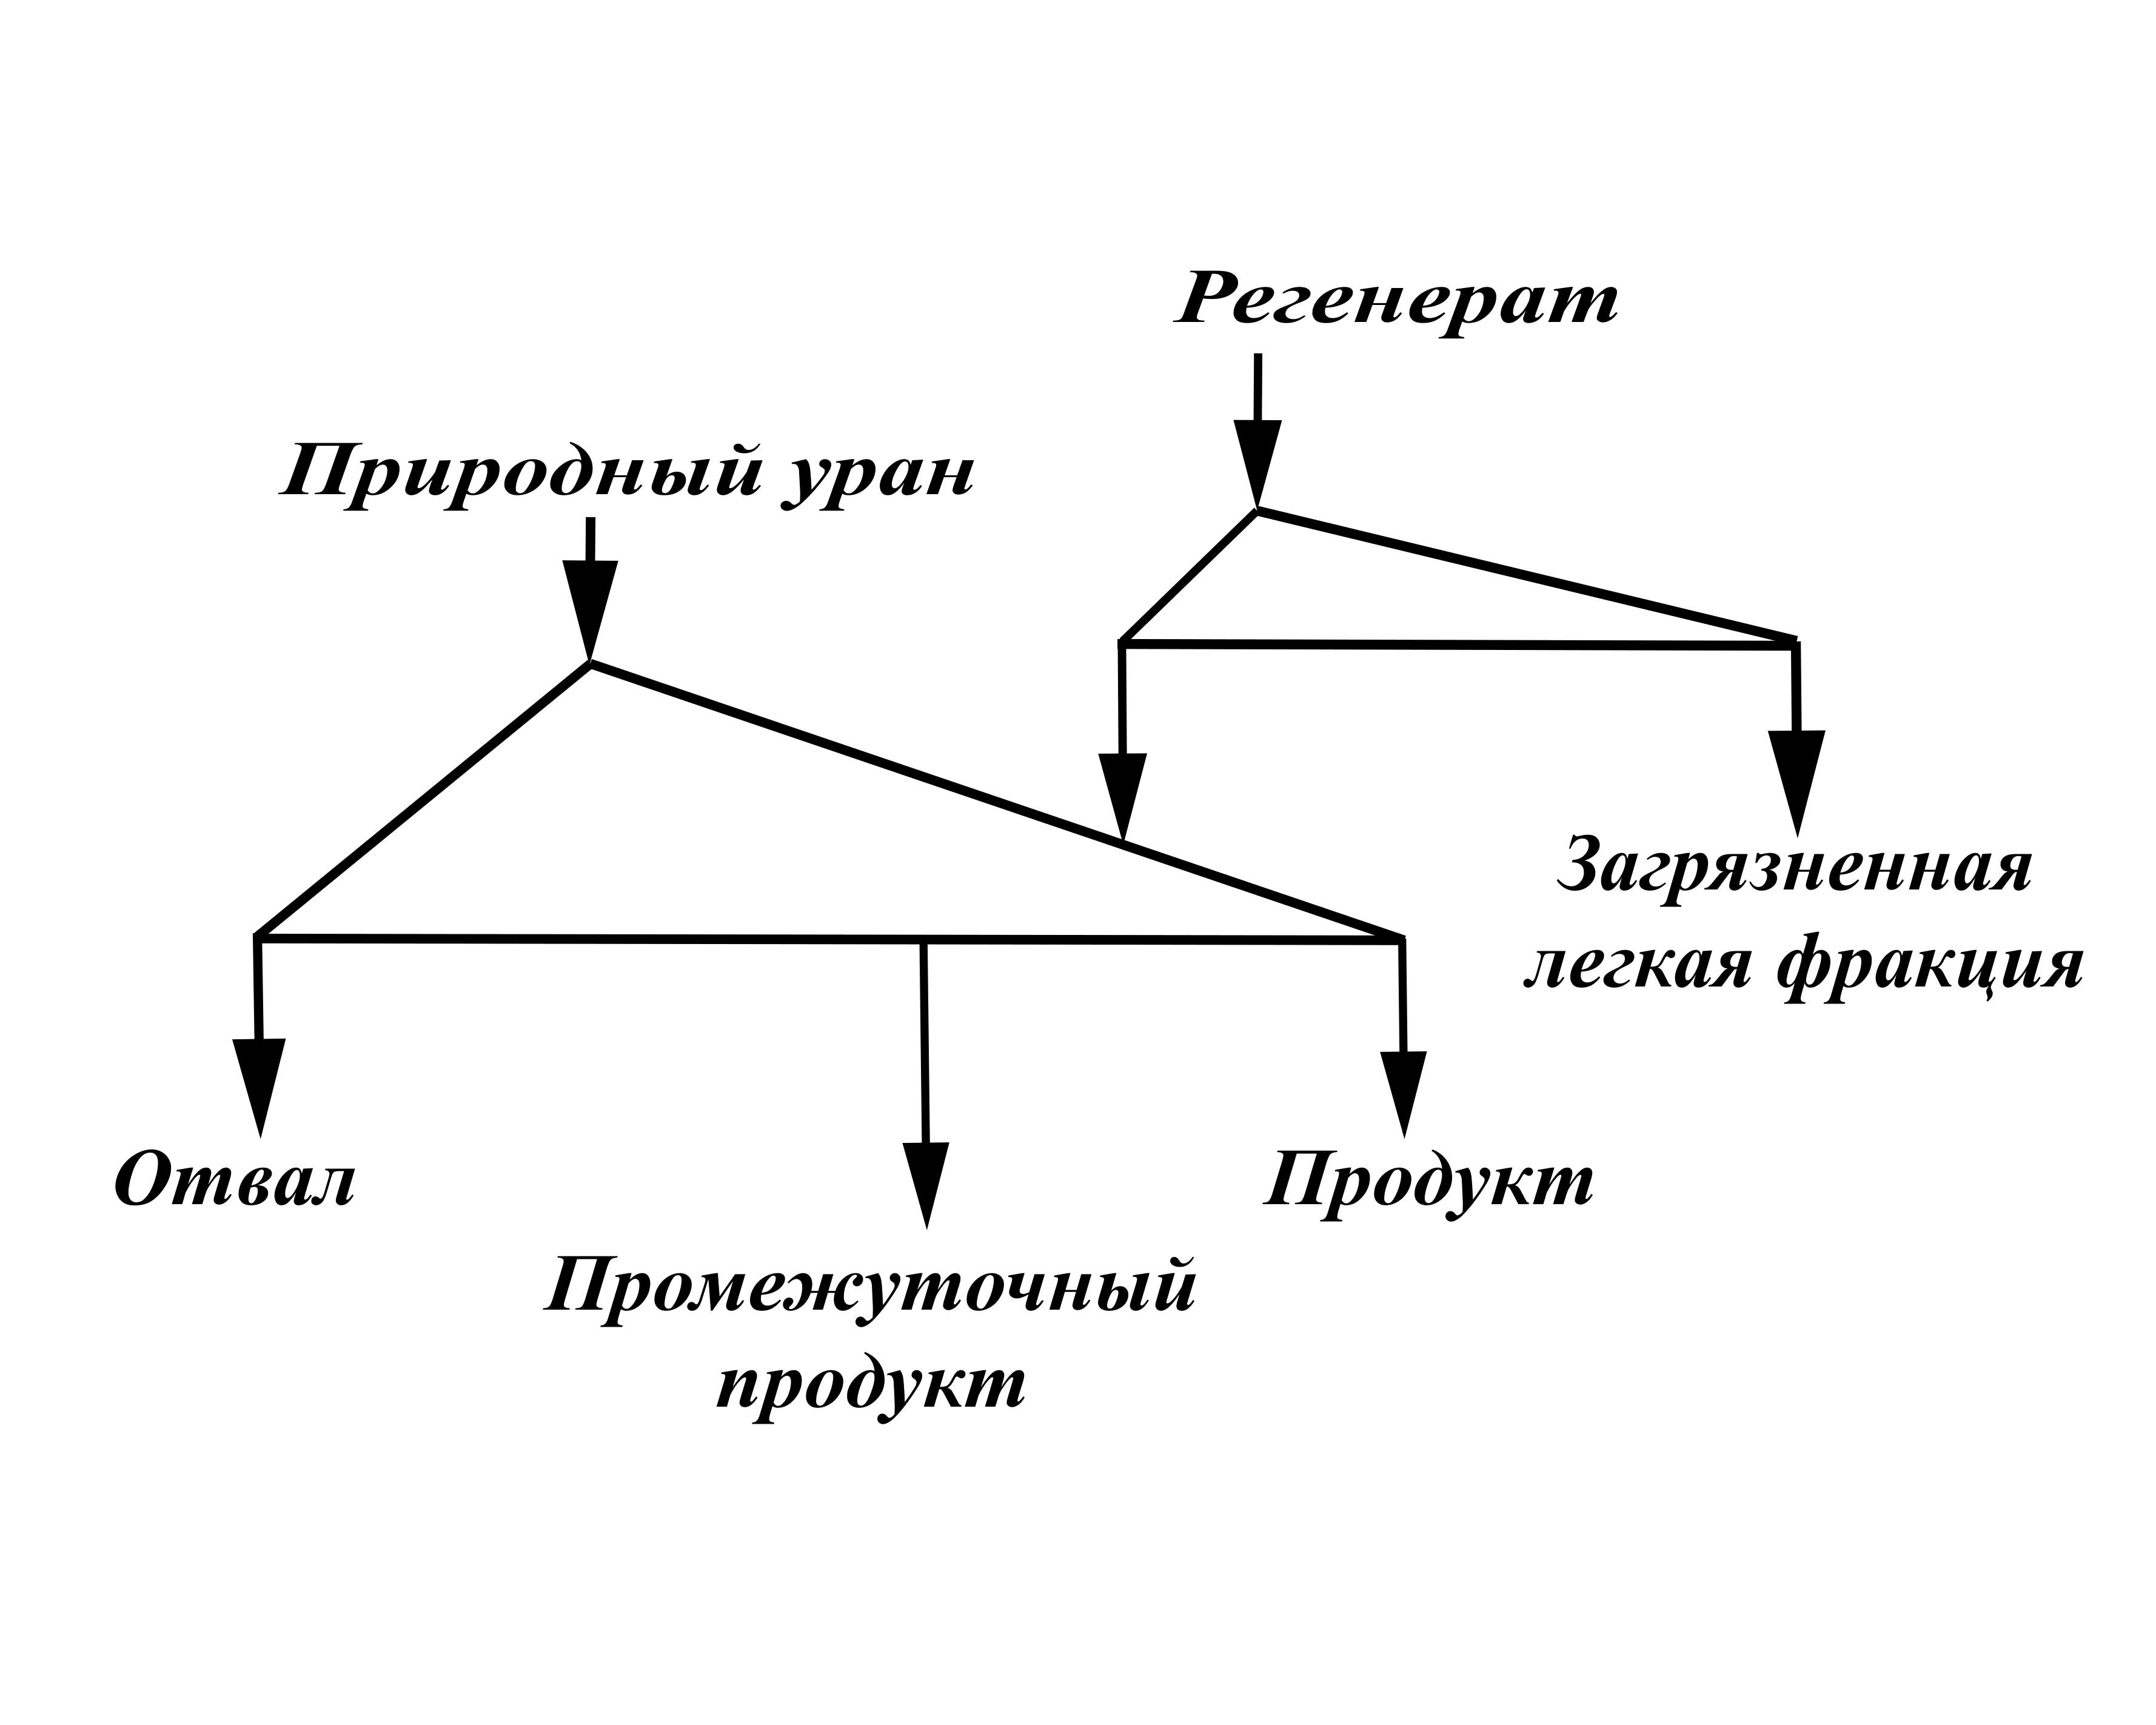
\includegraphics[scale=0.1]{cascades/double_palk}}
  \caption{Двойной каскад, использующий две стадии очистки}\label{fig:double_palk}
\end{figure}

Существует модификация двойного каскада, предложенная в \cite{smirnovDilutionRecycledUranium2015} использующая каскад с тремя питаниями  (рис. \ref{fig:double_3feeds}).
\begin{figure}[ht]
  \centerfloat{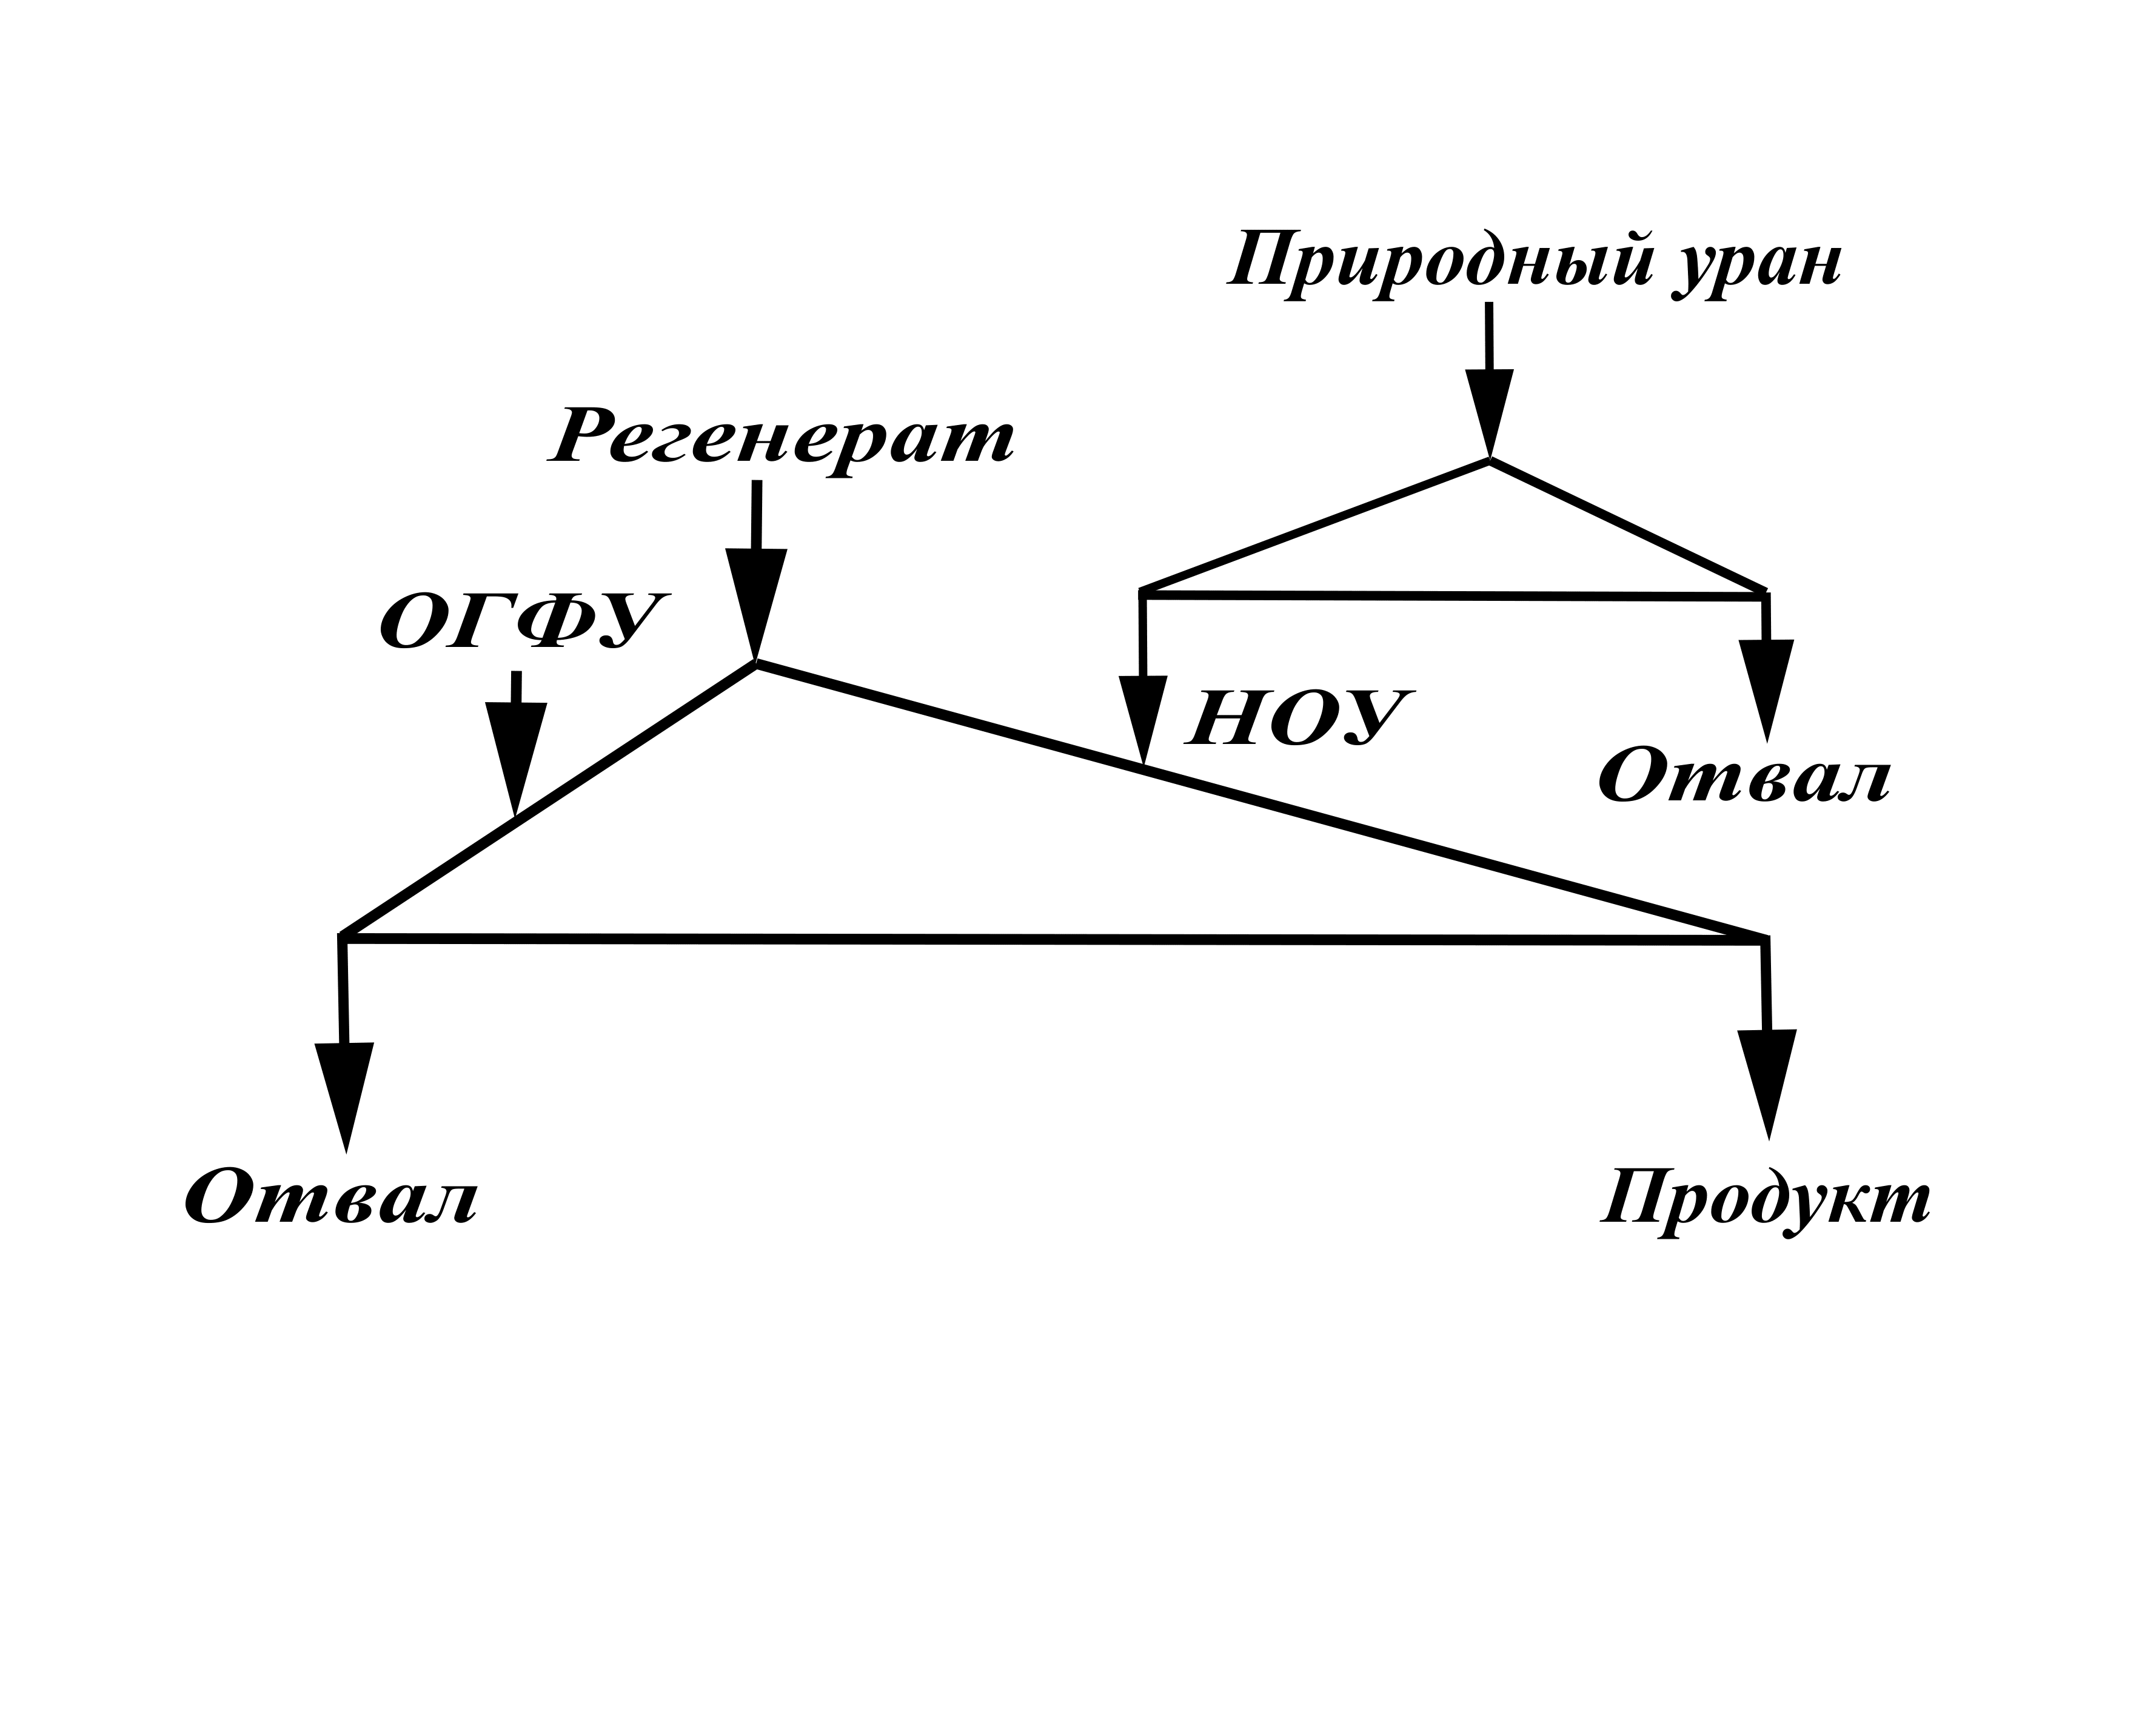
\includegraphics[scale=0.1]{cascades/double_3feeds}}
  \caption{Двойной каскад, использующий каскад с тремя питаниями}\label{fig:double_3feeds}
\end{figure}

Эта схема получила дальнейшее развитие в \cite{smirnovEvaluatingEffectivenessDilution2016}, где было продемонстрировано, что использование предварительно подготовленного низкообогащенного урана в качестве одного из питающих потоков, вместо использования природного урана, позволяет снизить себестоимость производства товарного НОУ-продукта.

Продолжая обзор примеров составных каскадных схем, рассмотрим способ производства изотопно-восстановленного регенерированного урана, предложенный в \cite{SposobIzotopnogoVosstanovleniyac}.

Принцип работы такой схемы состоит в том, что первый каскад (верхний на рис. \ref{fig:double_crazy}) обогащает регенерированный уран до $5,0-10,0$ по $^{232}$U, а потоки отвала и отбора направляются на питание второго каскада.
Изотопно восстановленный уран же производится во втором каскаде в потоке дополнительного отбора.
Этот промежуточный для производства НОУ продукт отбирается из промежуточной ступени второго каскада (рис. \ref{fig:double_crazy}).
\begin{figure}[ht]
  \centerfloat{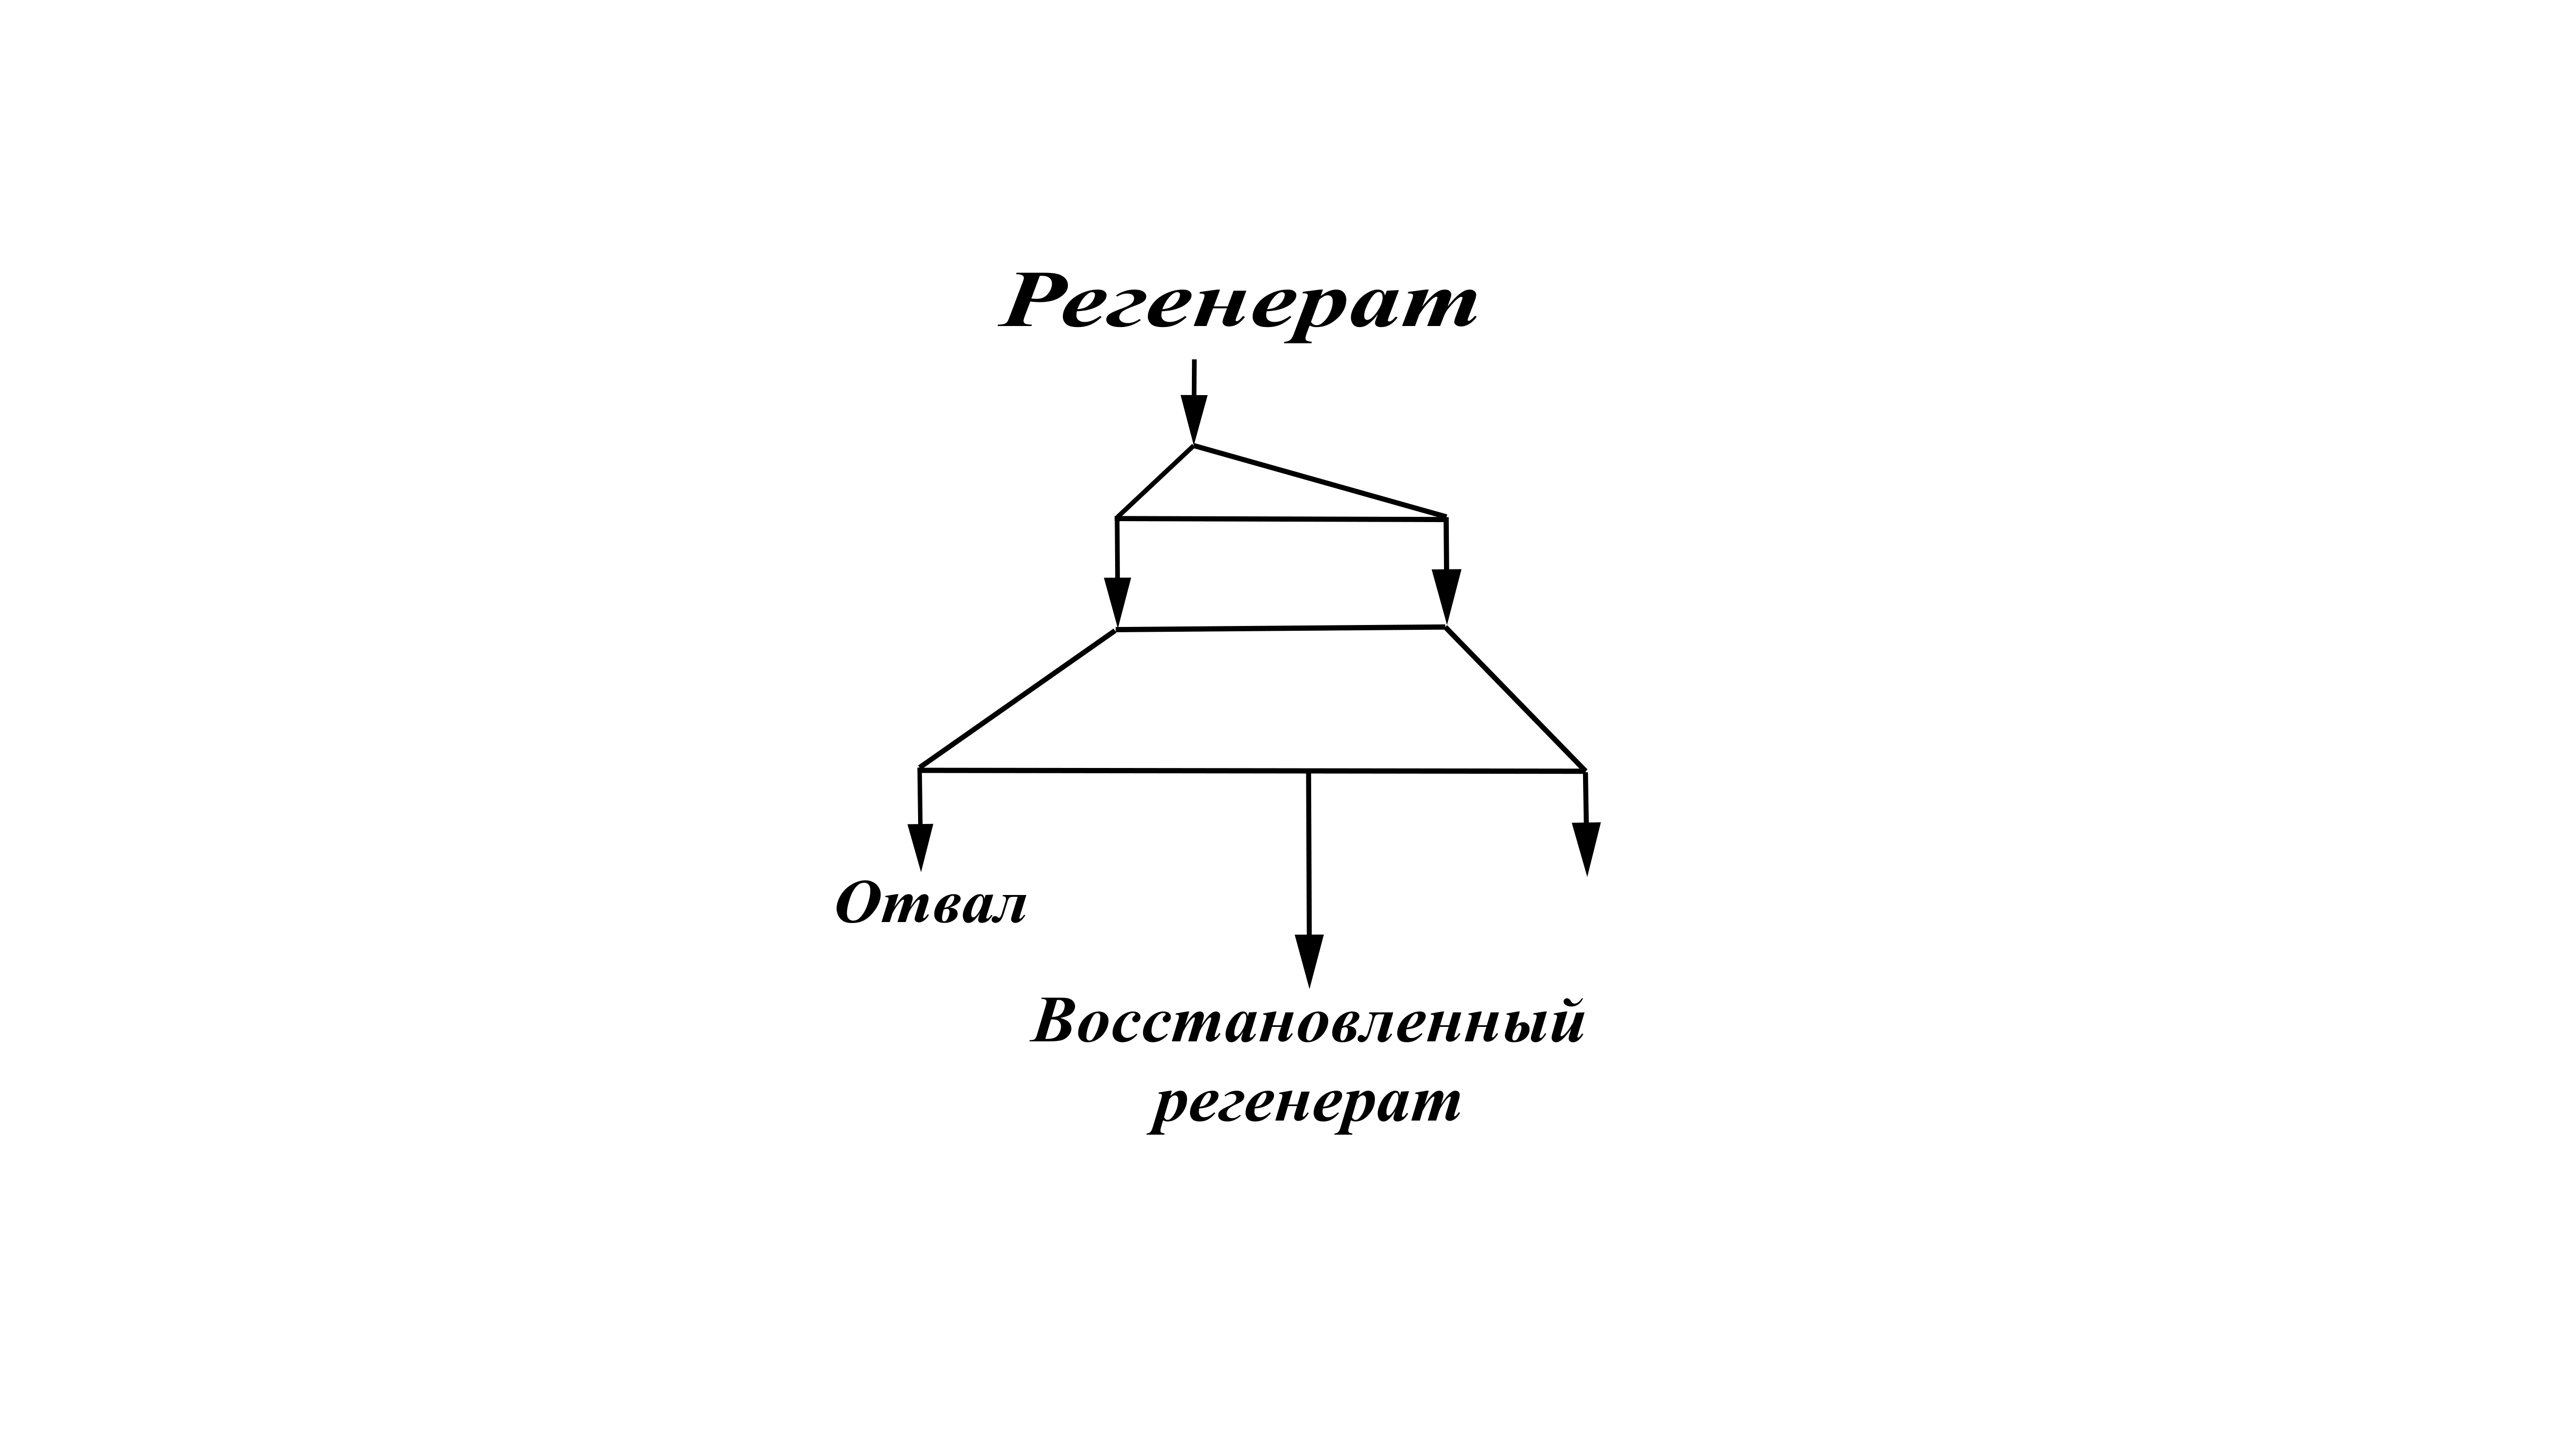
\includegraphics[scale=0.1]{cascades/double_crazy}}
  \caption{Двойной каскад, производящий восстановленный регенерат в промежуточном потоке отбора}\label{fig:double_crazy}
\end{figure}

По замыслу авторов, задачей изобретения является более полная очистка регенерата от $^{232}$U, при этом избегая операции разбавления скорректированного изотопного состава регенерированного урана ураном природного происхождения.
Однако, как и отмечают авторы, возможность извлечения $^{232}$U в такой схеме сильна ограничена.

Следует обратить особое внимание, что поток, произведенный в обогащающем ("легком") конце второго каскада, имеющий категорию ВОУ, не находит свое применение.
Этот изотопный состав смешивается с отвалом второго каскада, который позволяет экранировать гамма-излучение, обусловленное $^{232}$U.
Такое решение, по словам авторов, "минимизирует риски долговременного хранения невостребованных продуктов изотопной корректировки регенерированного урана".
То есть, это решение может быть использовано для устранения проблемы с потоком легкой фракции второго каскада схем, представленных на рис. \ref{fig:triple} и рис. \ref{fig:double_ru}.


Таким образом, изучение приведенных схем позволяет сделать выводы о физических принципах построения каскадов для решения задачи обогащения регенерата. 
Так, понимая закономерности массопереноса в каскадах, можно предложить конфигурацию, которая будет наилучшим образом подходить для решения сформулированной выше общей задачи обогащения регенерированного урана для получения НОУ товарного качества в условиях многократного рецикла топлива.

В качестве примера таких решений, существуют схемы, построенные с помощью синтеза ранее рассмотренных каскадов.
Такие схемы как изображенные на рис. \ref{fig:double_3feeds} и рис. \ref{fig:triple}) могут быть идеальным решением для некоторого класса задач, предоставляя уникальную гибкость в подстройке желаемых кровней экономии природного урана, работы разделения, или же задействования ОГФУ.

Таким образом, в построении схем могут использоваться полезные физические принципы, заимствованные из всего набора каскадов, предложенных в данном обзоре.

Как мы можем видеть на основании обзора составных каскадов, такие схемы очень перспективны как инструмент для возврата в ЯТЦ требуемого количества ОЯТ. Однако, 
так как мы нацелены на решение задачи обогащения регенерата в условиях многократного рецикла, а ни одна из существующего набора ранее предложенных схем, не может в полной мере решить поставленную задачу, возникает потребность дальнейших поисков. На них и направлена данная работа, которая предлагает в следующей главе (глава 2) выявить ограничения известных схем, чтобы предложить полезные модификации (глава 3).

